% Options for packages loaded elsewhere
\PassOptionsToPackage{unicode}{hyperref}
\PassOptionsToPackage{hyphens}{url}
\PassOptionsToPackage{dvipsnames,svgnames,x11names}{xcolor}
%
\documentclass[
  number,
  preprint,
  3p,
  onecolumn]{elsarticle}

\usepackage{amsmath,amssymb}
\usepackage{iftex}
\ifPDFTeX
  \usepackage[T1]{fontenc}
  \usepackage[utf8]{inputenc}
  \usepackage{textcomp} % provide euro and other symbols
\else % if luatex or xetex
  \usepackage{unicode-math}
  \defaultfontfeatures{Scale=MatchLowercase}
  \defaultfontfeatures[\rmfamily]{Ligatures=TeX,Scale=1}
\fi
\usepackage{lmodern}
\ifPDFTeX\else  
    % xetex/luatex font selection
\fi
% Use upquote if available, for straight quotes in verbatim environments
\IfFileExists{upquote.sty}{\usepackage{upquote}}{}
\IfFileExists{microtype.sty}{% use microtype if available
  \usepackage[]{microtype}
  \UseMicrotypeSet[protrusion]{basicmath} % disable protrusion for tt fonts
}{}
\makeatletter
\@ifundefined{KOMAClassName}{% if non-KOMA class
  \IfFileExists{parskip.sty}{%
    \usepackage{parskip}
  }{% else
    \setlength{\parindent}{0pt}
    \setlength{\parskip}{6pt plus 2pt minus 1pt}}
}{% if KOMA class
  \KOMAoptions{parskip=half}}
\makeatother
\usepackage{xcolor}
\setlength{\emergencystretch}{3em} % prevent overfull lines
\setcounter{secnumdepth}{5}
% Make \paragraph and \subparagraph free-standing
\ifx\paragraph\undefined\else
  \let\oldparagraph\paragraph
  \renewcommand{\paragraph}[1]{\oldparagraph{#1}\mbox{}}
\fi
\ifx\subparagraph\undefined\else
  \let\oldsubparagraph\subparagraph
  \renewcommand{\subparagraph}[1]{\oldsubparagraph{#1}\mbox{}}
\fi


\providecommand{\tightlist}{%
  \setlength{\itemsep}{0pt}\setlength{\parskip}{0pt}}\usepackage{longtable,booktabs,array}
\usepackage{calc} % for calculating minipage widths
% Correct order of tables after \paragraph or \subparagraph
\usepackage{etoolbox}
\makeatletter
\patchcmd\longtable{\par}{\if@noskipsec\mbox{}\fi\par}{}{}
\makeatother
% Allow footnotes in longtable head/foot
\IfFileExists{footnotehyper.sty}{\usepackage{footnotehyper}}{\usepackage{footnote}}
\makesavenoteenv{longtable}
\usepackage{graphicx}
\makeatletter
\def\maxwidth{\ifdim\Gin@nat@width>\linewidth\linewidth\else\Gin@nat@width\fi}
\def\maxheight{\ifdim\Gin@nat@height>\textheight\textheight\else\Gin@nat@height\fi}
\makeatother
% Scale images if necessary, so that they will not overflow the page
% margins by default, and it is still possible to overwrite the defaults
% using explicit options in \includegraphics[width, height, ...]{}
\setkeys{Gin}{width=\maxwidth,height=\maxheight,keepaspectratio}
% Set default figure placement to htbp
\makeatletter
\def\fps@figure{htbp}
\makeatother

\usepackage{lineno}\linenumbers \usepackage{multirow}
\makeatletter
\makeatother
\makeatletter
\makeatother
\makeatletter
\@ifpackageloaded{caption}{}{\usepackage{caption}}
\AtBeginDocument{%
\ifdefined\contentsname
  \renewcommand*\contentsname{Table of contents}
\else
  \newcommand\contentsname{Table of contents}
\fi
\ifdefined\listfigurename
  \renewcommand*\listfigurename{List of Figures}
\else
  \newcommand\listfigurename{List of Figures}
\fi
\ifdefined\listtablename
  \renewcommand*\listtablename{List of Tables}
\else
  \newcommand\listtablename{List of Tables}
\fi
\ifdefined\figurename
  \renewcommand*\figurename{Figure}
\else
  \newcommand\figurename{Figure}
\fi
\ifdefined\tablename
  \renewcommand*\tablename{Table}
\else
  \newcommand\tablename{Table}
\fi
}
\@ifpackageloaded{float}{}{\usepackage{float}}
\floatstyle{ruled}
\@ifundefined{c@chapter}{\newfloat{codelisting}{h}{lop}}{\newfloat{codelisting}{h}{lop}[chapter]}
\floatname{codelisting}{Listing}
\newcommand*\listoflistings{\listof{codelisting}{List of Listings}}
\makeatother
\makeatletter
\@ifpackageloaded{caption}{}{\usepackage{caption}}
\@ifpackageloaded{subcaption}{}{\usepackage{subcaption}}
\makeatother
\makeatletter
\@ifpackageloaded{tcolorbox}{}{\usepackage[skins,breakable]{tcolorbox}}
\makeatother
\makeatletter
\@ifundefined{shadecolor}{\definecolor{shadecolor}{rgb}{.97, .97, .97}}
\makeatother
\makeatletter
\makeatother
\makeatletter
\makeatother
\journal{Journal Name}
\ifLuaTeX
  \usepackage{selnolig}  % disable illegal ligatures
\fi
\usepackage[]{natbib}
\bibliographystyle{elsarticle-num}
\IfFileExists{bookmark.sty}{\usepackage{bookmark}}{\usepackage{hyperref}}
\IfFileExists{xurl.sty}{\usepackage{xurl}}{} % add URL line breaks if available
\urlstyle{same} % disable monospaced font for URLs
\hypersetup{
  pdftitle={Drought indices of water demand and supply, soil moisture, vegetation, and its impact on LULCC in continental Chile},
  pdfauthor={Francisco Zambrano},
  pdfkeywords={drought, land cover change, satellite},
  colorlinks=true,
  linkcolor={blue},
  filecolor={Maroon},
  citecolor={Blue},
  urlcolor={Blue},
  pdfcreator={LaTeX via pandoc}}

\setlength{\parindent}{6pt}
\begin{document}

\begin{frontmatter}
\title{Drought indices of water demand and supply, soil moisture,
vegetation, and its impact on LULCC in continental Chile}
\author[1]{Francisco Zambrano%
\corref{cor1}%
\fnref{fn1}}
 \ead{francisco.zambrano@umayor.cl} 

\affiliation[1]{organization={Universidad Mayor, Hémera Centro de
Observación de la Tierra, Facultad de Ciencias, Escuela de Ingeniería en
Medio Ambiente y Sustentabilidad},city={Santiago,
Chile},postcode={7500994},postcodesep={}}

\cortext[cor1]{Corresponding author}
\fntext[fn1]{This is the first author footnote.}
        
\begin{abstract}
Human-induced greenhouse gas emissions have increased the frequency
and/or intensity of weather and climate extremes. Central Chile has been
affected by a persistent drought which is impacting the hydrological
system and vegetation development. The region has been the focus of
research studies due to the diminishing water supply, this persistent
period of water scarcity has been defined as a ``mega drought''.
Nevertheless, our results evidence that the water deficit has expanded
beyond. Our goal is to analyze the impact of drought, measured by
drought indices of water supply/demand and vegetation status, in the
LULCC (land use land cover change) over continental Chile. For the
analysis, continental Chile was divided into five zones according to a
latitudinal gradient: ``Norte Grande'', ``Norte Chico'', ``Zona
Central'', ``Zona Sur'', and ``Zona Austral''. We used monthly climatic
re-analysis variables for precipitation, temperature and soil moisture
for 1981-2023 from ERA5-Land; and MODIS (Moderate-Resolution Imaging
Spectroradiometer) product MCD12Q1 for land cover for 2001-2021, and the
NDVI vegetation index from product MOD13A2 collection 6.1 for 2000-2023,
both from collection 6.1. We estimated atmospheric evaporative demand
(AED) by combining the Hargreaves-Samani equation with the ERA5-Land
temperature. We derived the drought indices SPI (Standardized
Precipitation Index), SPEI (Standardized Precipitation
Evapotranspiration Index), EDDI (Evaporative Demand Drought Index), zcSM
(standardized anomaly of cumulative soil moisture), and the zcNDVI
(standardized anomaly of cumulative NDVI). These indices were calculated
for time scales of 1, 3, 6, 12, 24, and 36 months, except for zcNDVI (1,
3, and 6 months). We analyzed the temporal correlation of SPI, SPEI,
EDDI, and zcSM with zcNDVI to have insights into the impact of water
supply and demand on vegetation. Our results showed that LULCC had an
increasing trend of 412 {[}km2yr−1{]} of forest expansion in the ``Zona
Sur'', together with a decreasing trend of 24 {[}km2yr−1{]} of cropland
contraction in the ``Zona Central'' meanwhile the ``Zona Sur'' showed an
increase of 31 {[}km2yr−1{]}, and a contraction of 80 {[}km2yr−1{]} of
bare soil in the ``Zona Austral''. The EDDI was the less correlated
index for the five macro zones and the five types of land cover, showing
that the temperature in Chile has little impact on vegetation. Higher
r-squared values, between 0.5 and 0.8, were obtained at ``Norte Chico''
and ``Zona Central'' for the land cover types of savanna, shrubland,
grassland, and croplands for the indices SPEI and zcSM at time scales of
12 and 24 months. The forest type reaches a r-squared of
\textasciitilde0.5 for zcSM of 12 months. The results indicate that the
``Norte Chico'' and ``Zona Central'' are the most sensitive regions to
water supply deficits longer than a year, potentially explained by a low
capacity of water storage in those zones that should be further
investigated.
\end{abstract}





\begin{keyword}
    drought \sep land cover change \sep 
    satellite
\end{keyword}
\end{frontmatter}
    \captionsetup{justification=raggedright,singlelinecheck=false}

\ifdefined\Shaded\renewenvironment{Shaded}{\begin{tcolorbox}[enhanced, frame hidden, boxrule=0pt, breakable, borderline west={3pt}{0pt}{shadecolor}, sharp corners, interior hidden]}{\end{tcolorbox}}\fi

\hypertarget{introduction}{%
\section{Introduction}\label{introduction}}

The sixth assessment report (AR6) of the IPCC \citep{IPCC2023} indicates
that human-induced greenhouse gas emissions have increased the frequency
and/or intensity of some weather and climate extremes, and the evidence
has been strengthened since AR5 \citep{IPCC2013}. There is high
confidence that increasing global warming can expand the land area
affected by increasing drought frequency and severity
\citep{IPCCCH112021}. Furthermore, drought increases tree mortality and
triggers changes in land cover and, consequently, land use, thus
impacting ecosystems \citep{Crausbay2017}. Nevertheless, there is a lack
of understanding of how the alteration in water supply and demand is
affecting land cover transformations.

Precipitation is the primary driver of drought and is intensified by
temperature \citep{Luo2017}. Drought impacts soil moisture, hydrological
regimes, and vegetation productivity. Initially, drought was commonly
classified as meteorological, hydrological, and agricultural
\citep{Wilhite1985}. Lately, \citep{Loon2016} and
\citep{AghaKouchak2021} have given an updated definition of drought for
the Anthropocene, suggesting that it should be considered the feedback
of humans' decisions and activities that drives the anthropogenic
drought. Even though it has been argued that those definitions do not
fully address the ecological dimensions of drought. \citep{Crausbay2017}
proposed the ecological drought definition as \emph{``an episodic
deficit in water availability that drives ecosystems beyond thresholds
of vulnerability, impacts ecosystem services, and triggers feedback in
natural and/or human systems''}. Moreover, many ecological studies have
misinterpreted how to characterize drought, for example, sometimes
considering ``dry'' conditions as ``drought'' \citep{Slette2019}. On the
other hand, the AR6 \citep{IPCC2023} states that even if global warming
is stabilized at 1.5°--2°C, many parts of the world will be impacted by
more severe agricultural and ecological droughts. Then, there is a
challenge in conducting drought research, especially to evaluate its
impact on ecosystems.

Chile has been facing a persistent rainfall deficit for more than a
decade \citep{Garreaud2017}, which has impacted vegetation development
\citep{Zambrano2023} and the hydrological system \citep{Boisier2018}.
Current drought conditions have affected crop productivity
\citep{Zambrano2016, Zambrano2018}, forest development
\citep{Miranda2020, Venegas2018}, forest fire occurrence
\citep{UrrutiaJalabert2018}, land cover change \citep{Fuentes2021},
water supply in watersheds \citep{AlvarezGarreton2021}, and have had
economic impacts \citep{Fernandez2023}. In 2019--2020, the drought
severity reached an extreme condition in Central Chile (30--34°S) not
seen for at least 40 years, and the evidence indicates that the impact
is transversal to the land cover classes of forest, grassland, and
cropland \citep{Zambrano2023}. The prolonged lack of precipitation in
Central Chile is producing changes in ecosystem dynamics that must be
studied.

For the spatiotemporal assessment of drought impact (i.e., by water
supply and demand) on land cover changes, we need climatic realiable
variables such as precipitation, temperature, soil moisture, land cover,
and vegetation status. For developing countries like Chile, the weather
networks present several disadvantages, such as gaps, a short history,
and low-quality data. Reanalysis data, as the ERA5-Land (ERA5L)
\citep{MunozSabater2021} provides hourly climatic information
(precipitation, temperature, and soil moisture) without gaps since 1950
with global extension. ERA5L has already been used for drought
assessment using the Standardized Precipitation-Evapotranspiration Index
(SPEI) \citep{Nouri2023} and for flash drought \citep{Wang2023} by
analyzing soil mositure and evapotranspiration. On the other hand,
satellite remote sensing \citep{West2019, AghaKouchak2015} is the
primary method to evaluate how drought impacts vegetation dynamics.
Vegetation drought indices (VDI) are commonly used as proxies of
productivity \citep{Paruelo2016, Schucknecht2017}, which can be derived
from the MODIS (Moderate-Resolution Imaging Spectroradiometer). Besides,
land use and land cover (LULC) change can be driven by drought
\citep{Tran2019, Akinyemi2021}. To analyze these changes, multiple LULC
products exist \citep{Grekousis2015}, one of those that provides time
series since 2001 is the MCD12Q1 \citep{Friedl2019} from MODIS. The
variation in water supply and demand is finally reflected in the total
water storage (TWS). The TWS can be retrieved by the Gravity Recovery
and Climate Experiment (GRACE), which allows analyzing water
availability changes at coarse resolution \citep{Ahmed2014, Ma2017}. We
can use climatic reanalysis (ERA5L) and vegetation data (MODIS) to
derive drought indices of supply (i.e., precipitation) and demand (i.e.,
temperature) and thus evaluate the impact of drought on LULC changes.
Further, the TWS can be assessed with regard to the changes in water
supply and demand to gain insight into the impact on water storage.

To evaluate meteorological drought (i.e., water supply), the World
Meteorological Organization (WMO; \citep{WMO2012}) recommends the
Standardized Precipitation Index (SPI; \citep{Mckee1993}), a multiscalar
drought index that allows to monitor precipitation deficits from short-
to long-term. Following the same approach, \citep{Vicente-Serrano2010}
incorporates into the SPI the effect of temperature through the use of
potential evapotranspiration, thus proposing the SPEI (Standardized
Precipitation Evapotranspiration Index). Similarly, to evaluate solely
the evaporative demand driven by temperature, \citep{Hobbins2016} and
\citep{McEvoy2016} came up with the Evaporative Demand Drought Index
(EDDI). For vegetation, in a similar manner as the SPI, SPEI and EDDI;
\citep{Zambrano2018} proposed the zcNDVI, a standardized anomaly of the
cumulative Normalized Difference Vegetation Index (NDVI), which could be
acumulated over the growing season or any period (e.g., months),
resulting in a multiscalar drought index. For soil moisture, several
drought indices exist, such as the Soil Moisture Deficit Index (SDMI) a
normalized index \citep{Narasimhan2005} and the Soil Moisture
Agricultural Drought Index (SMADI) \citep{Souza2021} which is a
normalized index using vegetation, land surface temperature, and a
vegetation condition index (VCI, \citep{Kogan1995}). From TWS, we can
estimate the standardized terrestrial water storage index (STI)
\citep{Cui2021}, a standardized anomaly that follows the methodology of
the SPI, SPEI, EDDI, and zcNDVI. Thereby, we have drought indices for
water supply, demand, and storage, which can help to make a
comprehensive assessment of drought.

In this research, we present the raster dataset DDS4Chl, which provides
climate variables and drought indices of water demand and supply and
vegetation productivity for continental Chile since 1981 at a monthly
frequency. Those were gathered from the earth observation products
ERA5-Land and MODIS. Then, we used DDS4Chl to analyze the impact of
drought on different types of land cover classes in continental Chile.
The specific objectives of the study are: i) to analyze the trend on
multi-scalar drought indices for water demand and supply, soil moisture,
and vegetation productivity for 1981--2023/2001--2023; ii) to evaluate
LULC change for 2001--2021 and its relation to drought indices; iii) to
analyze the relationship of a proxy of vegetation productivity (zcNDVI)
with drought indices of water demand and supply and soil moisture; and
iv) to assess if the observed changes in the drought indices are linked
to TWS.

\hypertarget{study-area}{%
\section{Study area}\label{study-area}}

Continetal Chile has a diverse climate condition from north to south and
east to west \citep{Aceituno2021} (Figure~\ref{fig-studyArea}), which
determines its great ecosystem diversity (Figure~\ref{fig-LCprop}). The
Andes Mountains are a main factor in latitudinal variation
\citep{Garreaud2009}. To describe the climate and ecosystem of Chile, we
use the Koppen-Geiger release by \citep{Beck2023} and the landcover type
persistance of 80\% of times for 2001--2022, from the IGBP
classification scheme \citep{Friedl2019} (see
Section~\ref{sec-methods_lulc}). ``Norte Grande'' and ``Norte Chico''
predominate in an arid desert climate with hot (Bwh) and cold (Bwk)
temperatures. At the south of ``Norte Chico,'' the climate changes to an
arid steppe with cold temperatures (Bsk). Mainly, the land is barren,
with a minor surface of vegetation types such as shrubland and
grassland. In the zones ``Centro'' and the north half of ``Sur,'' the
main climate is Mediterranean, with warmer to hot summers (Csa and Csb).
In ``Centro,'' there is a major proportion (\textasciitilde50\%) of
chilean matorral (shrubland and savanna), followed by grassland
(\textasciitilde16\%), forest (8\%), and croplands (5\%). The south part
of ``Centro'' and the north part of ``Austral'' are dominated by an
Oceanic climate (Cfb). Those zones are high in forest and grassland. The
southern part of the country has a tundra climate, and in Patagonia, it
is a cold semi-arid area with an extended surface of grassland.

\begin{figure}[!ht]

{\centering 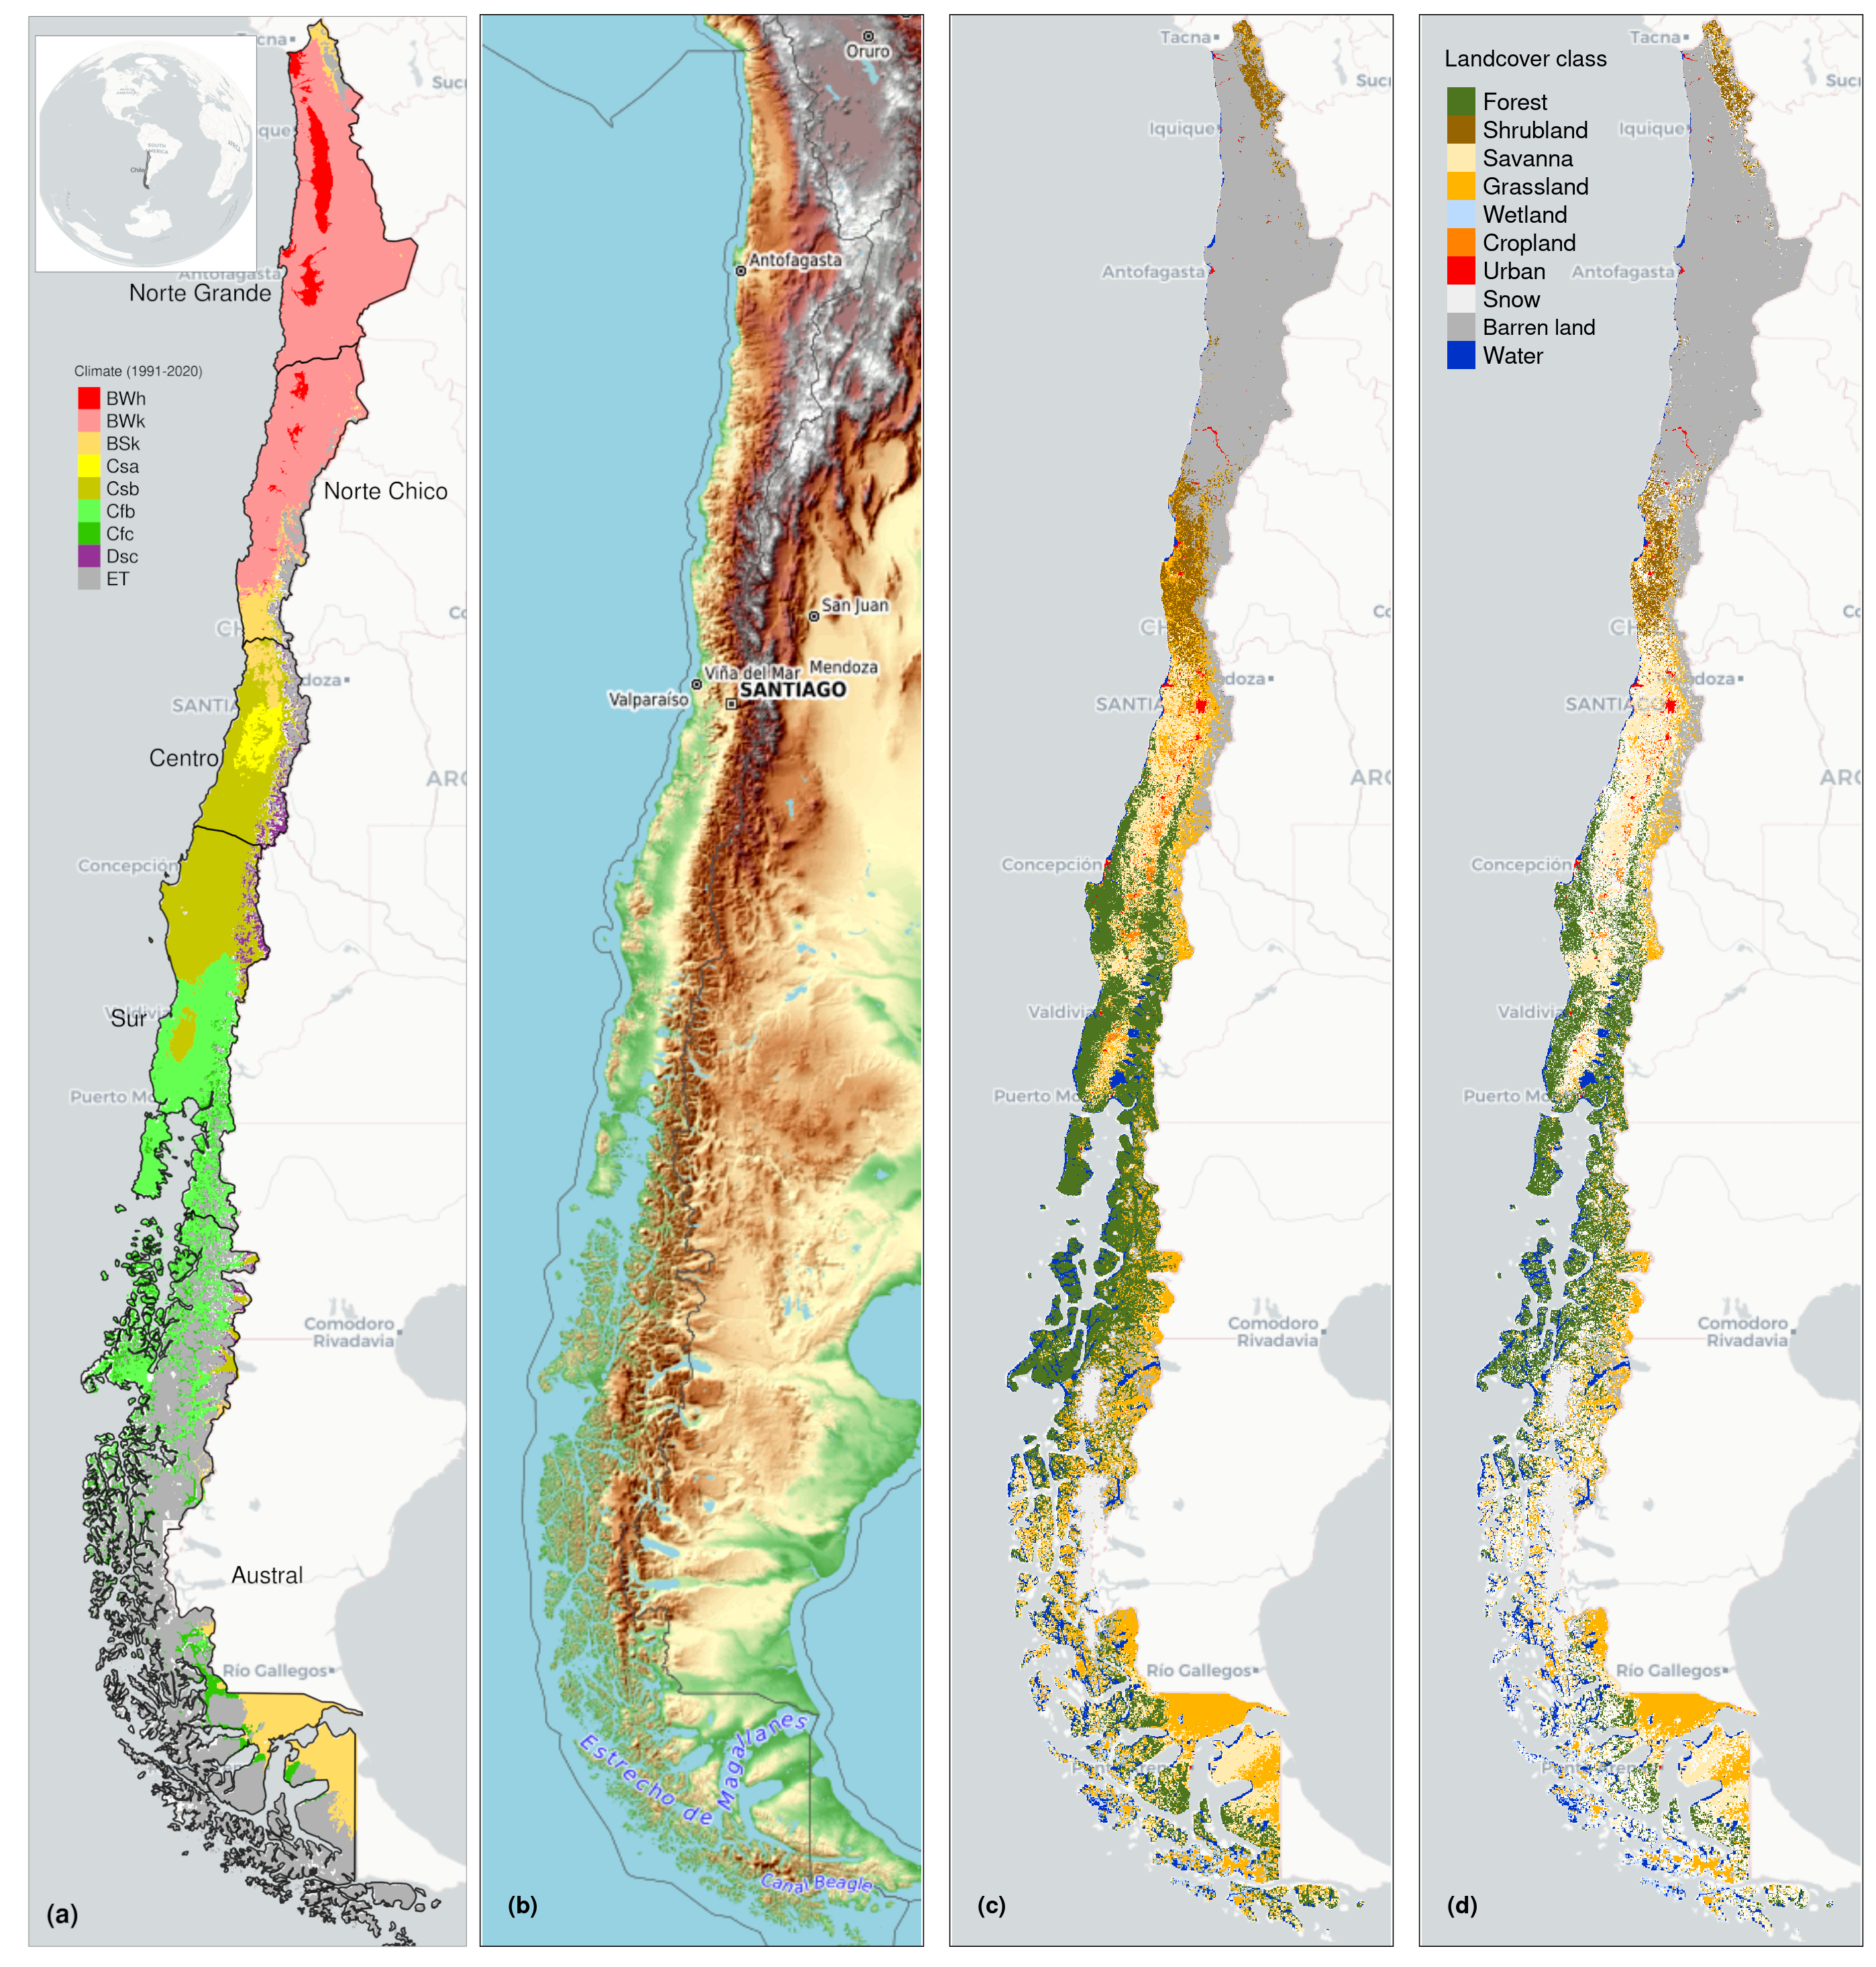
\includegraphics{../output/figs/map_study_con_landcover.png}

}

\caption{\label{fig-studyArea}(a) Chile with the Koppen-Geiger climate
classes and the five macrozones ``Norte Grande'', ``Norte Chico'',
``Centro'', ``Sur'', and ``Austral''. (b) Topography reference map. (c)
Land cover classes for 2022. (d) Persistent land cover classes
(\textgreater{} 80\%) for 2001-2022}

\end{figure}

\hypertarget{materials-and-methods}{%
\section{Materials and Methods}\label{materials-and-methods}}

\hypertarget{data}{%
\subsection{Data}\label{data}}

\hypertarget{earth-observation-data}{%
\subsubsection{Earth observation data}\label{earth-observation-data}}

For water supply and demand variabes, we used ERA5-Land
\citep{MunozSabater2021}, a reanalys dataset wich provides the evolution
of land variables since 1950. It has a spatial resolution of 0.1°,
hourly frequency and global coverage. We selected the variables for
total precipitation, 2 meters temperature maximum and minimum, and
volumetric soil water layers between 0 and 100cm of depth (layer 1 to
layer 3).

To derive a proxy of vegetation productivity, we used the product
MOD13A3 collection 6.1 from MODIS \citep{Didan2015}. It provides
vegetation indices (NDVI and EVI) at 1km of spatial resolution and
monthly frequency.

\begin{table}[!ht]
\caption{Description of the earth observation data used }
\label{tab-desEOD}
\small
\centering
\begin{tabular}{p{0.13\textwidth}cp{0.3\textwidth}p{0.095\textwidth}ccc}
\hline
\multirow{1}{*}{\centering Product} & Sub-product & Variable & Spatial Resolution  & Period & Units & Short Name \\ 
\hline
\multirow{4}{*}{ERA5-Land} & ~ & Precipitation & \multirow{4}{*}{~0.1°} & \multirow{4}{*}{1981-2023} & mm & P \\ 
         &  & Maximum temperature & ~ & & $°C$ & $T_{max}$ \\ 
         &  & Minimum temperature & ~ & & $°C$ & $T_{min}$ \\ 
         &  & Volumetric Soil Water Content at 1m & ~ & & $m3/m3$ & SM \\ 
ERA5-Land* & & Atmospheric Evaporative Demand & 0.1° & 1981-2023 & mm & AED \\
        \multirow{2}{*}{MODIS} & MOD13A3.061 & Normalized Difference Vegetation Index & \multirow{2}{*}{~1 km} & 2000-2023 & ~ & NDVI \\ 
         & MCD12Q1.061 & Landcover IGBP scheme & & 2001-2022 & ~ & Landcover \\ 
\hline
\end{tabular}
{\raggedright *Derived from ERA5-Land with Eq. \ref{eq-AED}. \par}
\end{table}

\hypertarget{in-situ-data}{%
\subsubsection{in-situ data}\label{in-situ-data}}

\hypertarget{software-and-packages-used}{%
\subsection{Software and packages
used}\label{software-and-packages-used}}

For the downloading, processing, and analysis of the spatio-temporal
data, we used the open source software for statistical computing and
graphics, \texttt{R} \citep{R2023}. For downloading ERA5-Land, we used
the \texttt{\{ecmwfr\}} package \citep{Hufkens2019}. For processing
raster data, we used \texttt{\{terra\}} \citep{Hijmans2023} and
\texttt{\{stars\}} \citep{Pebesma2023}. For managing vectorial data, we
used \texttt{\{sf\}} \citep{Pebesma2018}. For the calculation of AED, we
used \texttt{\{SPEI\}} \citep{Bergueria2023}.

\hypertarget{drought-indices}{%
\subsection{Drought Indices}\label{drought-indices}}

We derived the drought indices of water supply and demand, soil moisture
from the ERA5-Land dataset, and vegetation from the MODIS product, all
at monthly frequency.

For the indices EDDI and SPEI that use water demand, first we have to
calculate the AED. For this, we used the method of Hargreaves
\citep{Hargreaves1994}:

\begin{equation}\protect\hypertarget{eq-AED}{}{AED = 0.0023\cdot Ra\cdot (T+17.8)\cdot (T_{max}-T_{min})^{0.5}}\label{eq-AED}\end{equation}

where \(Ra\) \((MJ\,m^2\, day^{-1})\) is extraterrestrial radiation;
~\(T\), \(T_{max}\), and \(T_{min}\) are mean, maximum, and minimum
temperature \((°C)\). We calculate the centroid coordinates per pixel
and use the latitude to estimate \(Ra\).

To evaluate water demand, we chose the \(EDDI\)
\citep{Hobbins2016, McEvoy2016} index, which uses the \(AED\). For
supply, we used the index recommended by the World Meteorological
Organization (WMO) for monitoring drought, the SPI \citep{Mckee1993}. We
calculated the SPEI, which used a balance between \(P\) and \(AED\), in
this case, an auxiliary variable \(D = P-AED\) is used. In this study,
we propose the \(zcSM\) (standardized anomaly of acumulated soil
moisture at 1 m), which uses SM. Finally, for the proxy of productivity,
\(zcNDVI\), we used the NDVI. Before using the NDVI, it was smoothed
following the procedure described in \citep{Zambrano2018} and
\citep{Zambrano2016}.

All the indices are multi-scalar and were calculated for time scales of
1, 3, 6, 12, 24, and 36 months, except for zcNDVI, which was calculated
for 6 months. The goal is to be able to evaluate short- and long-term
droughts in water demand and supply and soil moisture. This is
particularly important for central Chile because it has suffered from a
prolonged decrease in precipitation for more than 12 years
\citep{Garreaud2020, Boisier2018, Garreaud2017}.

To calculate the drought indices, first we must calculate the
accumulation of the variable. In this case, for generalization purposes,
we will use \(V\), referring to \(P\), \(AED\), \(D\), \(NDVI\), and
\(SM\) (Table \ref{tab-desEOD}). We cumulated each \(V\) over the time
series of \(n\) values, and for the time scales \(s\):

\begin{equation}\protect\hypertarget{eq-sumvar}{}{A_{si} = \sum_{i=n-s-i+2}^{n-i+1} V_i\,\, \forall\, i\geq n-s+1  }\label{eq-sumvar}\end{equation}

It corresponds to a moving window (convolution) that sums the variable
for \(s\) starting for the last month \(n\) until the month, which could
sum for \(s\) months (n-s+1). Once the variable is cumulated over time
for the scale \(s\), we used a nonparametric approach following
\citep{Hobbins2016} to derive the drought indices. Thus, the empirically
derived probabilities are obtained through an inverse normal
approximation \citep{Abramowitz1968}. Then, we used the empirical Tukey
plotting position \citep{Wilks2011} over \(A_i\) to derive the
\(P(A_i)\) probabilities across a period of interest:

\begin{equation}\protect\hypertarget{eq-probPai}{}{P(A_i) = \frac{i-0.33}{n+0.33'}}\label{eq-probPai}\end{equation}

The drought indices \(SPI\), \(SPEI\), \(EDDI\), \(zcSM\), and
\(zcNDVI\) are obtained following the inverse normal approximation:

\begin{equation}\protect\hypertarget{eq-DI}{}{DI(A_i) = W - \frac{C_0+C_1\cdot W + c_2 \cdot W^2}{1+d_1\cdot W +d_2\cdot W^2 +d_3\cdot W^3}}\label{eq-DI}\end{equation}

\(DI\) is referring to the drought index calculated for the variable
\(V\). The values for the constats are: \(C_0 = 2.515517\),
\(C_1 = 0.802853\), \(C_2 = 0.010328\), \(d_1 = 1.432788\),
\(d_2 = 0.189269\), and \(d3 = 0.001308\). For \(P(A) \leq 0.5\),
W=\(\sqrt{-2\cdot ln(P(A_i))}\) , and for \(P(A_i) > 0.5\), replace
\(P(A_i)\) with \(1-P(A_i)\) and reverse the sign of \(DI(A_i)\).

\hypertarget{trend-of-drought-indices-for-water-demand-and-supply-soil-moisture-and-vegetation-productivity}{%
\subsection{Trend of drought indices for water demand and supply, soil
moisture, and vegetation
productivity}\label{trend-of-drought-indices-for-water-demand-and-supply-soil-moisture-and-vegetation-productivity}}

To estimate if there are significant positive or negative trends for the
drought indices, we used the non-parametric test of Mann-Kendall
\citep{Kendall1975}. To determine the magnitude of the trend, we used
Sen's slope \citep{Sen1968}. One of the advantages of applying this
methodology is that the Sen's slope is not affected by outliers as
regular regression does. We applied both to the five indices at the six
time scales from 1981 to 2023 and indices SPI, EDDI, SPEI, and zcSM, and
from 2000 to 2023 in the case of zcNDVI.

\citep{Vicente-Serrano2021} made a global analysis of the drought's
severity trend using SPI, SPEI, and the Standardized Evapotranspiration
Deficit Index (SEDI; \citep{Vicente-Serrano2018}) to evaluate AED. They
indicate that the increase in hydrological drought has been due to
anthropogenic effects rather than climate change. This is because the
global increase in AED does not explain the change in the spatial
pattern of hydrological drought. Also, they state that \emph{``the
increase in hydrological droughts has been primarily observed in regions
with high water demand and land cover change''}. We will contrast this
hypothesis with what is occurring in Chile. To achieve this, we will use
the landcover class type that remain more than 80\% of types for
2001-2022, and use this as a mask, where there are low changes, to
evaluate the trend on zcNDVI.

\hypertarget{sec-methods_lulc}{%
\subsection{LULC change for 2001-2022 and its relation with water supply
and demand, and soil moisture}\label{sec-methods_lulc}}

\begin{figure}[!ht]

{\centering 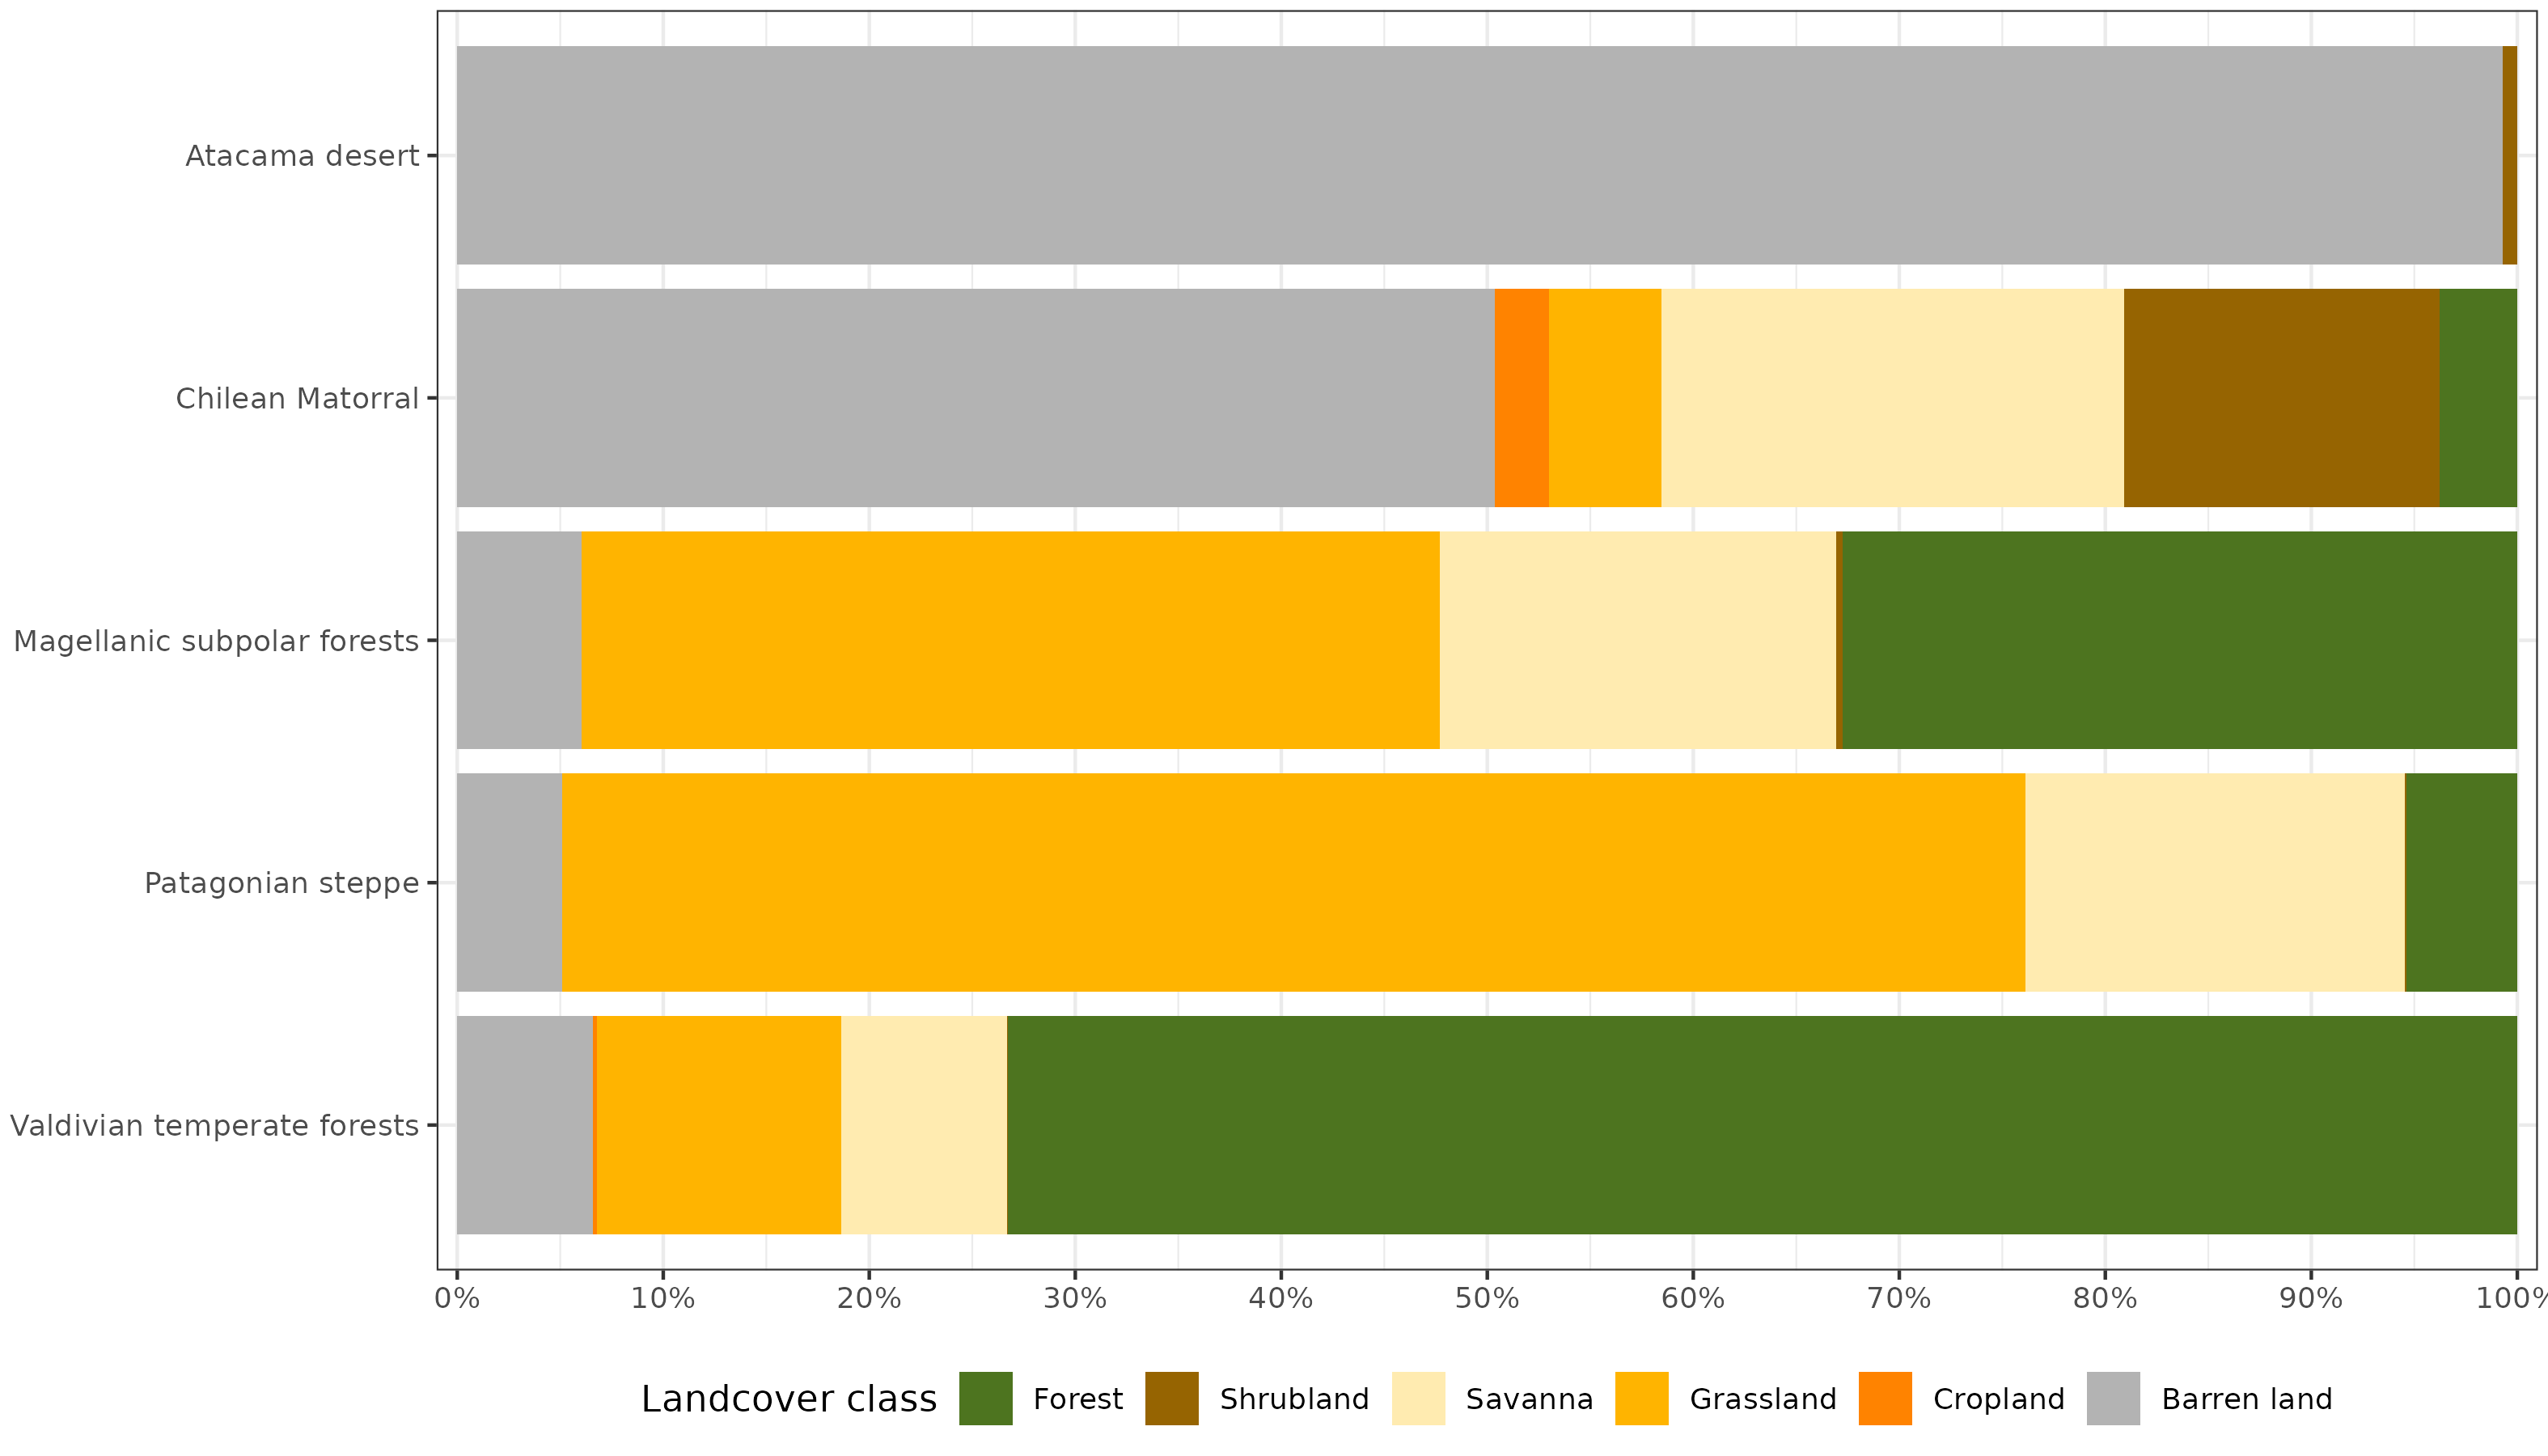
\includegraphics{../output/figs/LC_pers80_per_macrozone.png}

}

\caption{\label{fig-LCprop}Proportion of land cover class from the
persistent land cover for 2001-2022 (\textgreater80\%) per macrozone}

\end{figure}

To analyze the LULCC, we use the IGBP scheme from the MCD12Q1 collection
6.1 from MODIS. This product has a yearly frequency from 2011 to 2022.
The IGBP defines 17 classes; from these, we regrouped into ten
macroclasses for forest, schrublands, savannas, grasslands, wetlands,
croplands, urban, snow and ice, barren, and water bodies. Then, we
calculated the surface ocuppied per landcover class into each macrozone
(``Norte Grande'' to ``Austral'') per year. To determine the trend of
change we used the Sen' slope \citep{Sen1968} over the surface per year.

We calculated a raster mask considering the classes that remains more
than 80\% of years (2001-2022), which allow us to identify the areas
with no landcover change for the macroclasses. Figure~\ref{fig-LCprop}
shows the summary of proportion of surface per landcover class and
macrozone, derived from the mask over continental Chile.

We will explore if the trend in landcover classess is associated to
trend of the drought indices. For this we will use the regularizations
techniques of Lasso \citep{Tibshirani2010} and Ridge regressión
\citep{Hoerl1970}. Also, we will test random forest for this purpose
\citep{Ho1995}.

\hypertarget{impact-for-water-supply-and-demand-and-soil-moisture-in-vegetation-productivity-within-landcover-types}{%
\subsection{Impact for water supply and demand, and soil moisture in
vegetation productivity within landcover
types}\label{impact-for-water-supply-and-demand-and-soil-moisture-in-vegetation-productivity-within-landcover-types}}

The aim of this section is to analyze the drought indices of water
demand and supply and soil moisture against vegetation to address: i) if
short- or long-term time scales are most important in impacting
vegetation through Chile; and ii) the strength of the correlation for
the variable and the time scale. Then, we will summarize for each
landcover class and macrozone. Thus, we will be able to advance in
understanding how climate is affecting vegetation, considering the
impact on the five macroclasses: forest, cropland, grassland, savanna,
and shrubland.

To assess how water demand and supply and soil moisture are related to
vegetation productivity (zcNDVI), we analyze the linear correlation
between the indices SPI, SPEI, EDDI, and zcSM for 1, 3, 6, 12, 24, and
36-month time scales against zcNDVI. We followed a similar approach to
that used by \citep{Meroni2016} when using the SPI for meteorological
drought against the cumulative FAPAR (Fraction of Absorbed
Photosynthetically Active Radiation) as a proxy for vegetation
productivity. We made a pixel-to-pixel linear correlation analysis per
index. First, we calculate the Pearson coefficient of correlation for
the six time scales and let the time scale that reaches the maximum
correlation be significant (p \textless{} 0.05). Then, we extracted the
Pearson correlation value corresponding to the time scales that reached
the maximum value. Thus, we derived two raster maps per index, the first
with the time scales and the second with the correlation value.

\hypertarget{validation-of-era5-land-variables}{%
\subsection{Validation of ERA5-Land
variables}\label{validation-of-era5-land-variables}}

\hypertarget{results}{%
\section{Results}\label{results}}

\hypertarget{trend-of-drought-indices-for-water-demandsupply-soil-moisture-and-vegetation-productivity}{%
\subsection{Trend of drought indices for water demand/supply, soil
moisture, and vegetation
productivity}\label{trend-of-drought-indices-for-water-demandsupply-soil-moisture-and-vegetation-productivity}}

Regarding vegetation productivity, there is a negative trend on zcNDVI
in the central part of the country (``norte chico'' and ``zona
central'') (Figure~\ref{fig-zcNDVI_var}). Indicating either a reduction
of vegetation surface, biomass, or status. It reached its lowest values
during the year 2020, mostly on the ``zona central.'' There are other
negative trends in small areas in ``norte grande'' and ``zona asutral.''

\begin{figure}[!ht]

{\centering 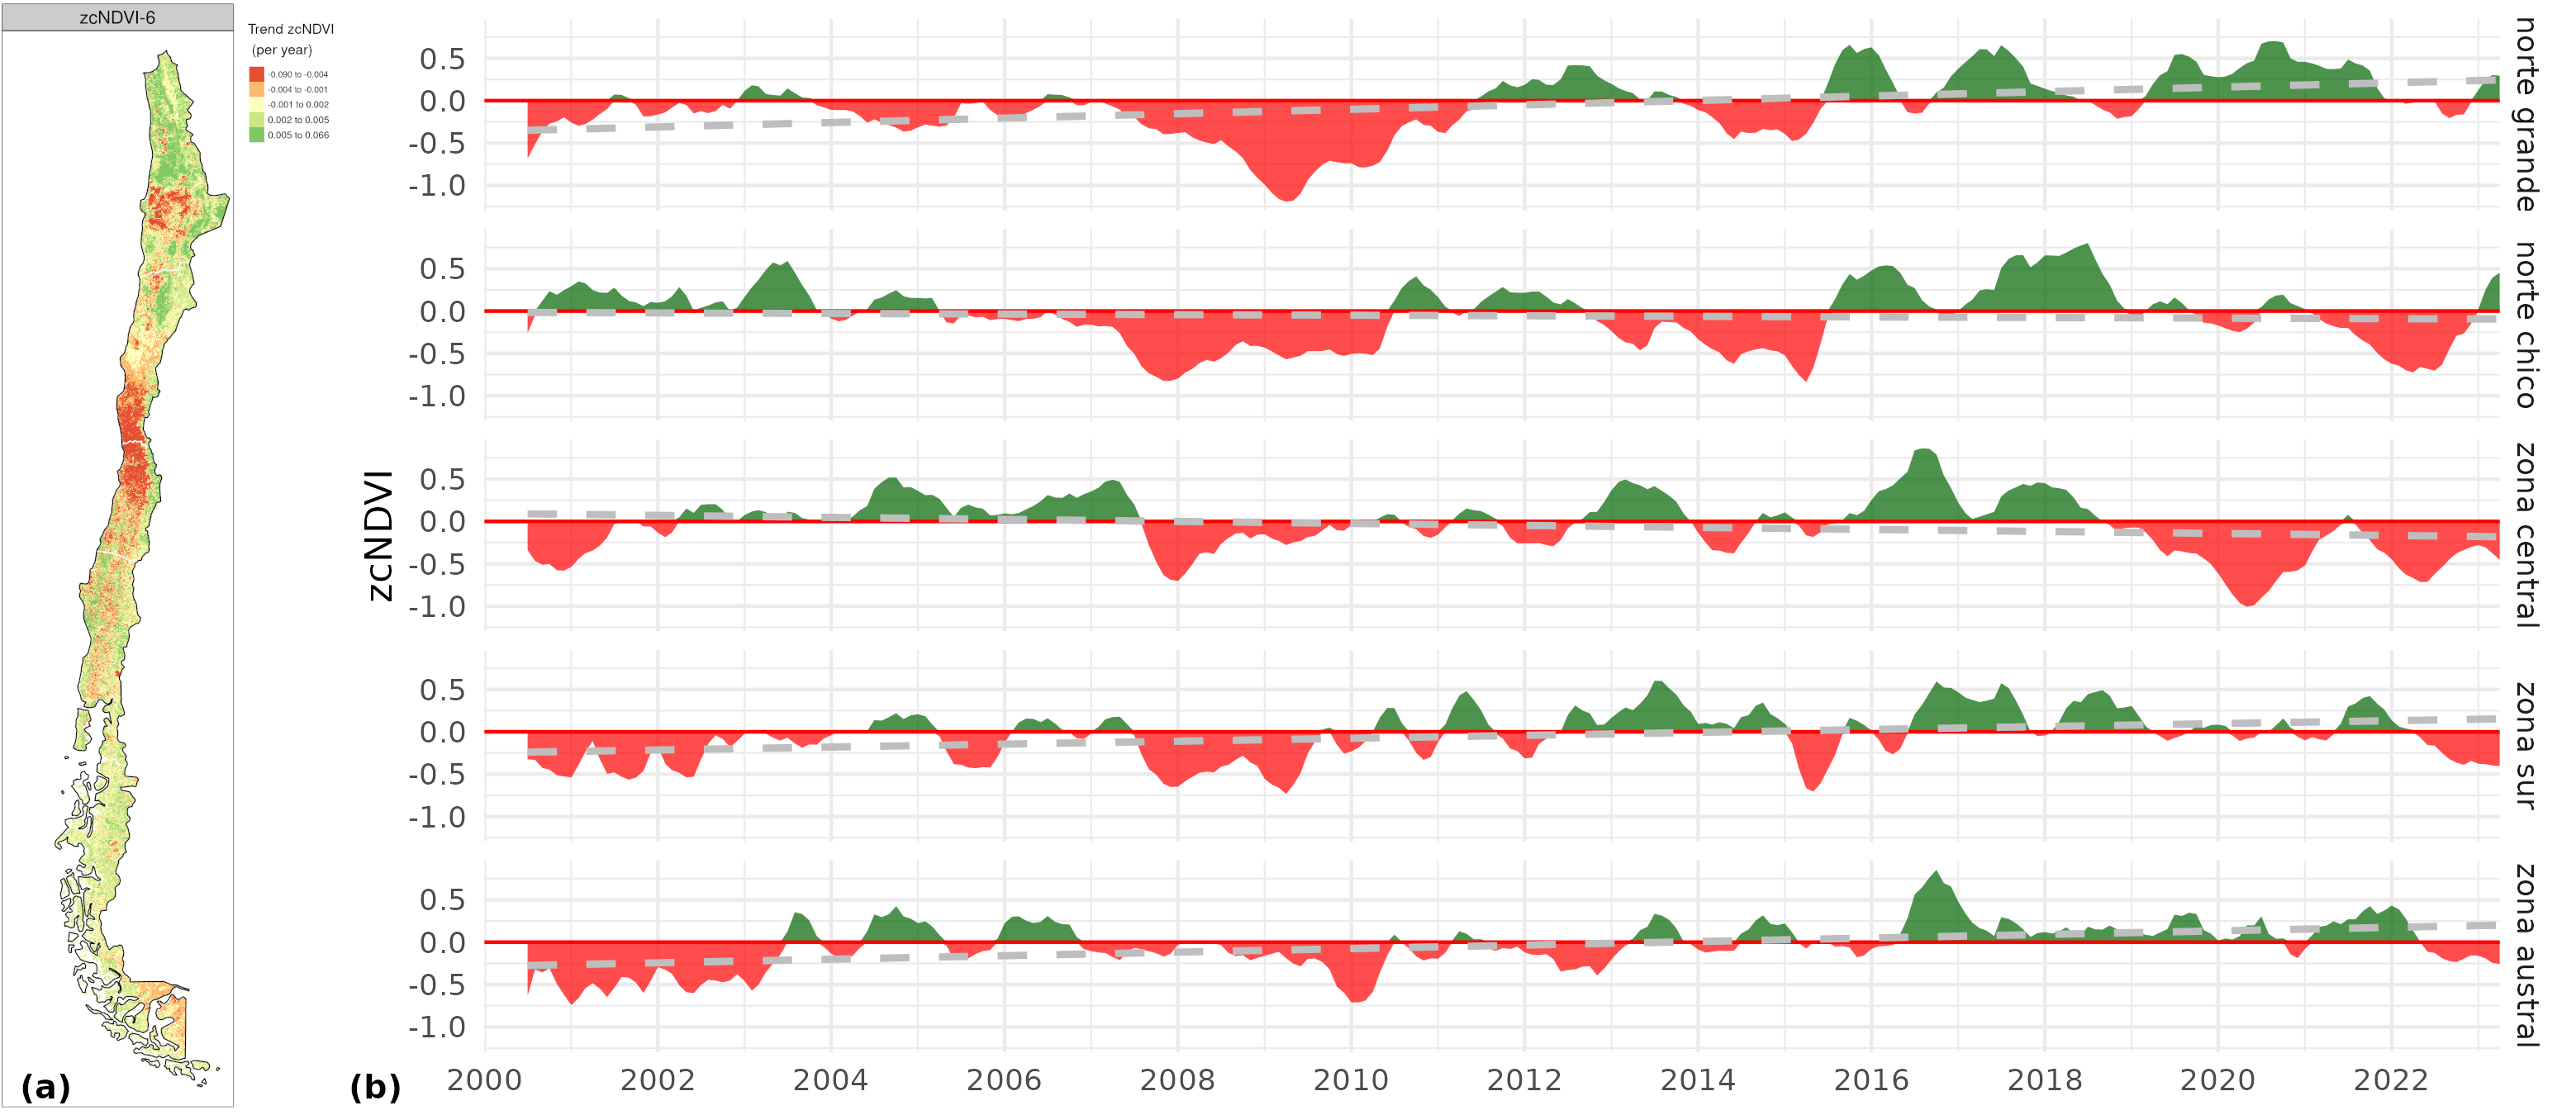
\includegraphics{../output/figs/temporal_variation_zcNDVI6_macrozonas.png}

}

\caption{\label{fig-zcNDVI_var}(a) Map of the linear trend of the index
zcNDVI-6 for 2001--2023. Greener colors indicate a positive trend and an
increase in vegetation development; reder colors correspond to a
negative trend and a decrease in vegetation development. (b) Temporal
variation of zcNDVI-6 aggregated at macrozone level within continental
Chile. Each horizontal panel corresponds to a macrozone from `norte
grande' to `zona austral'.}

\end{figure}

Analyzing the water supply in the macrozones ``norte chico,''
``central,'' and ``sur,'' the SPI shows a decreasing trend that
increases at longer time scales due to the prolonged reduction in
precipitation. It reaches a trend of -0.056 (z-score) per decade
(Figure~\ref{fig-trendSPI}) for time scales of 36 months. In the case of
water demand, we analyze the EDDI. It shows a positive trend, caused by
an increase in AED. The trend on EDDI reaches a maximum of 0.053 per
decade in the macrozones ``norte grande'' and ``norte chico''
(Figure~\ref{fig-trendEDDI}). The behavior is similar to SPI, having
close trends with opposite signs. Nevertheless, the spatial patterns are
different. The maximum trend for SPI-36 is in ``norte chico'' and ``zona
central.'' For EDDI-36, the maximum trend is from ``northe grande'' to
``zona central.''

\begin{figure}[!ht]

{\centering 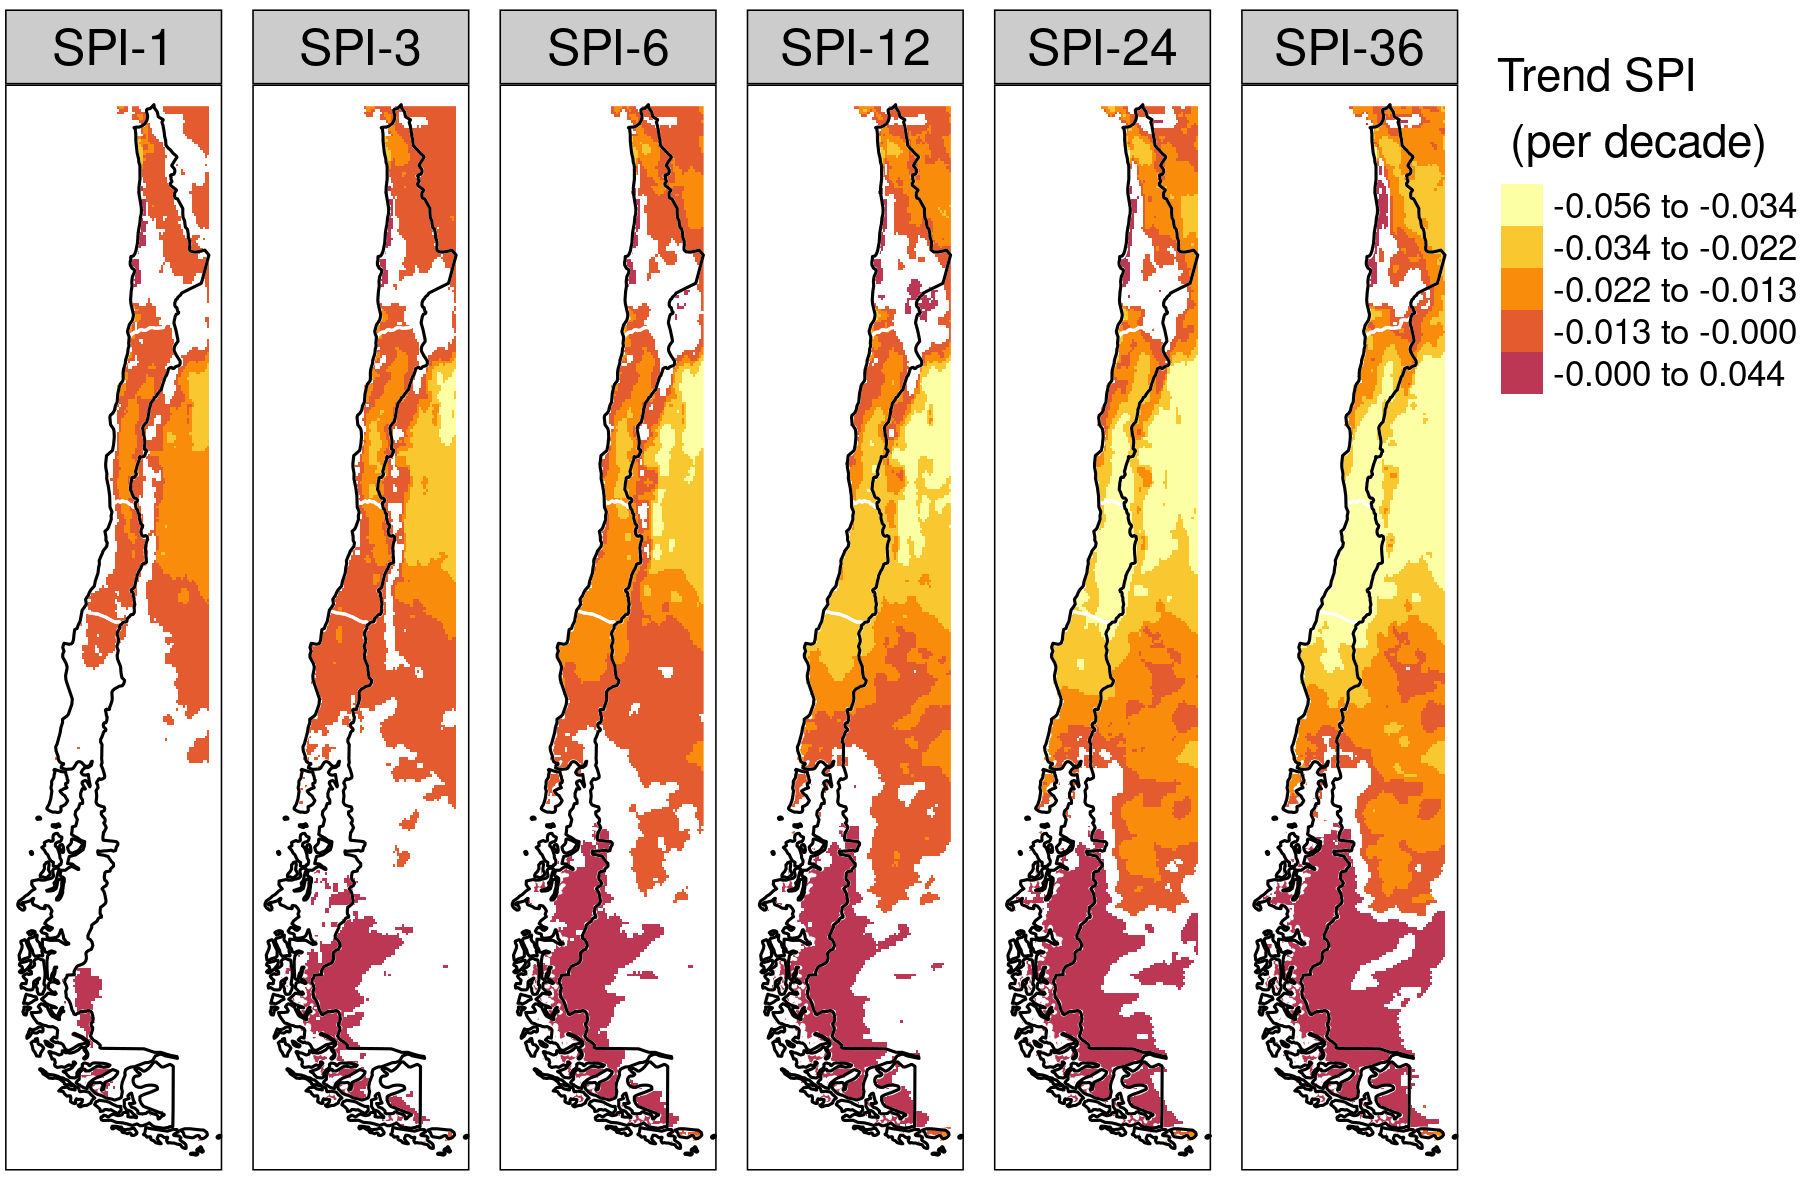
\includegraphics{../output/figs/trend_raster_SPI_1981-2023.png}

}

\caption{\label{fig-trendSPI}Linear trend of the SPI at time scales of
1, 3, 6, 12, 24, and 36 months for 1981-2023}

\end{figure}

\begin{figure}[!ht]

{\centering 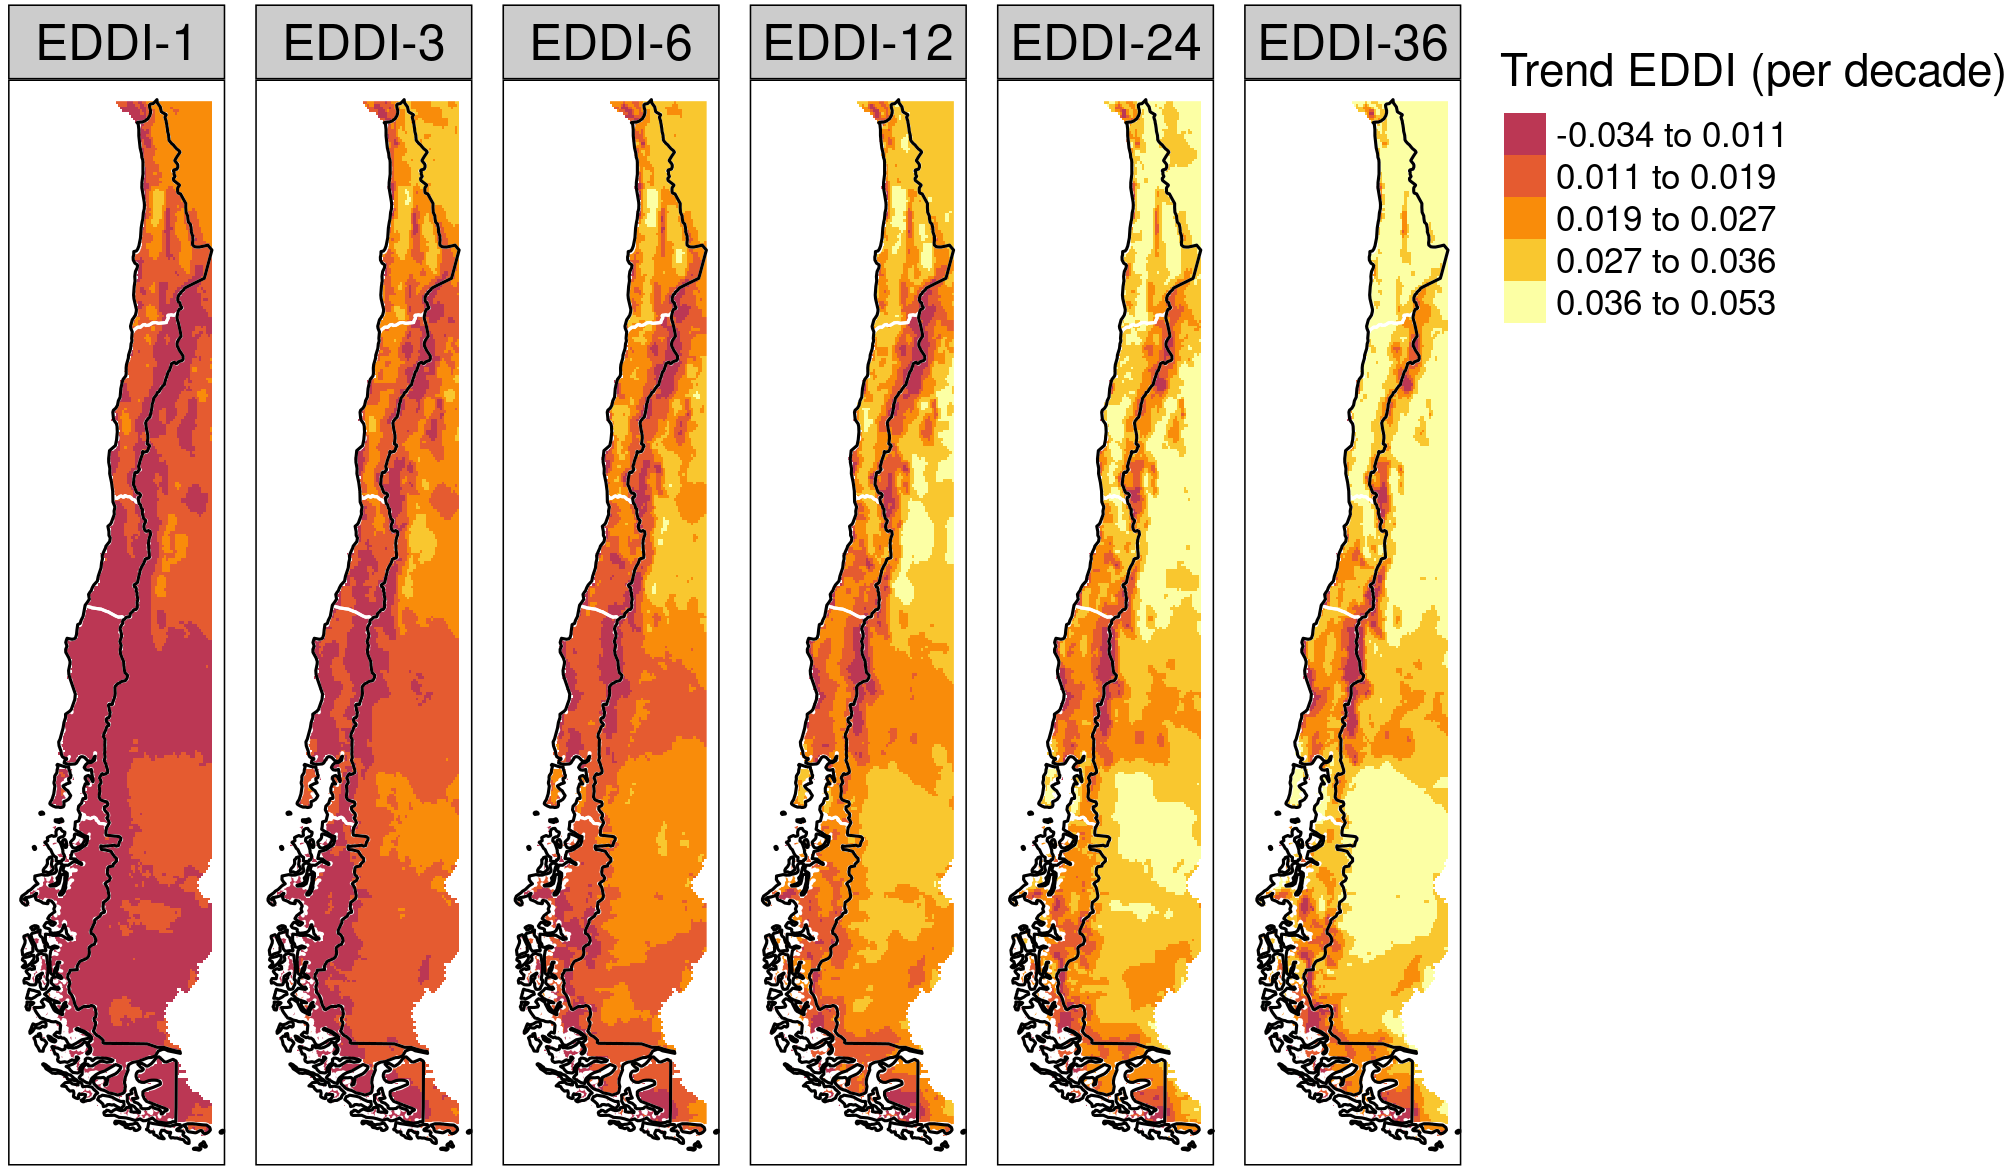
\includegraphics{../output/figs/trend_raster_EDDI_1981-2023.png}

}

\caption{\label{fig-trendEDDI}Linear trend of the EDDI at time scales of
1, 3, 6, 12, 24, and 36 months for 1981-2023}

\end{figure}

The correlation between zcNDVI-6 and drought indices shows that time
scales higher than six months are predominant over continental Chile in
explaining vegetation variability (Figure~\ref{fig-corTimeScale}).
Pearson correlations between 0.6 and 0.9 are concentrated in the ``norte
chico'' and ``zona central'' for SPI and SPEI. Soil moisture reached a
correlation of 0.6--0.9 that extended north and south with respect to
SPI.

\hypertarget{impact-for-water-supply-and-demand-and-soil-moisture-in-vegetation-productivity}{%
\subsection{Impact for water supply and demand, and soil moisture in
vegetation
productivity}\label{impact-for-water-supply-and-demand-and-soil-moisture-in-vegetation-productivity}}

\begin{figure}[!ht]

{\centering 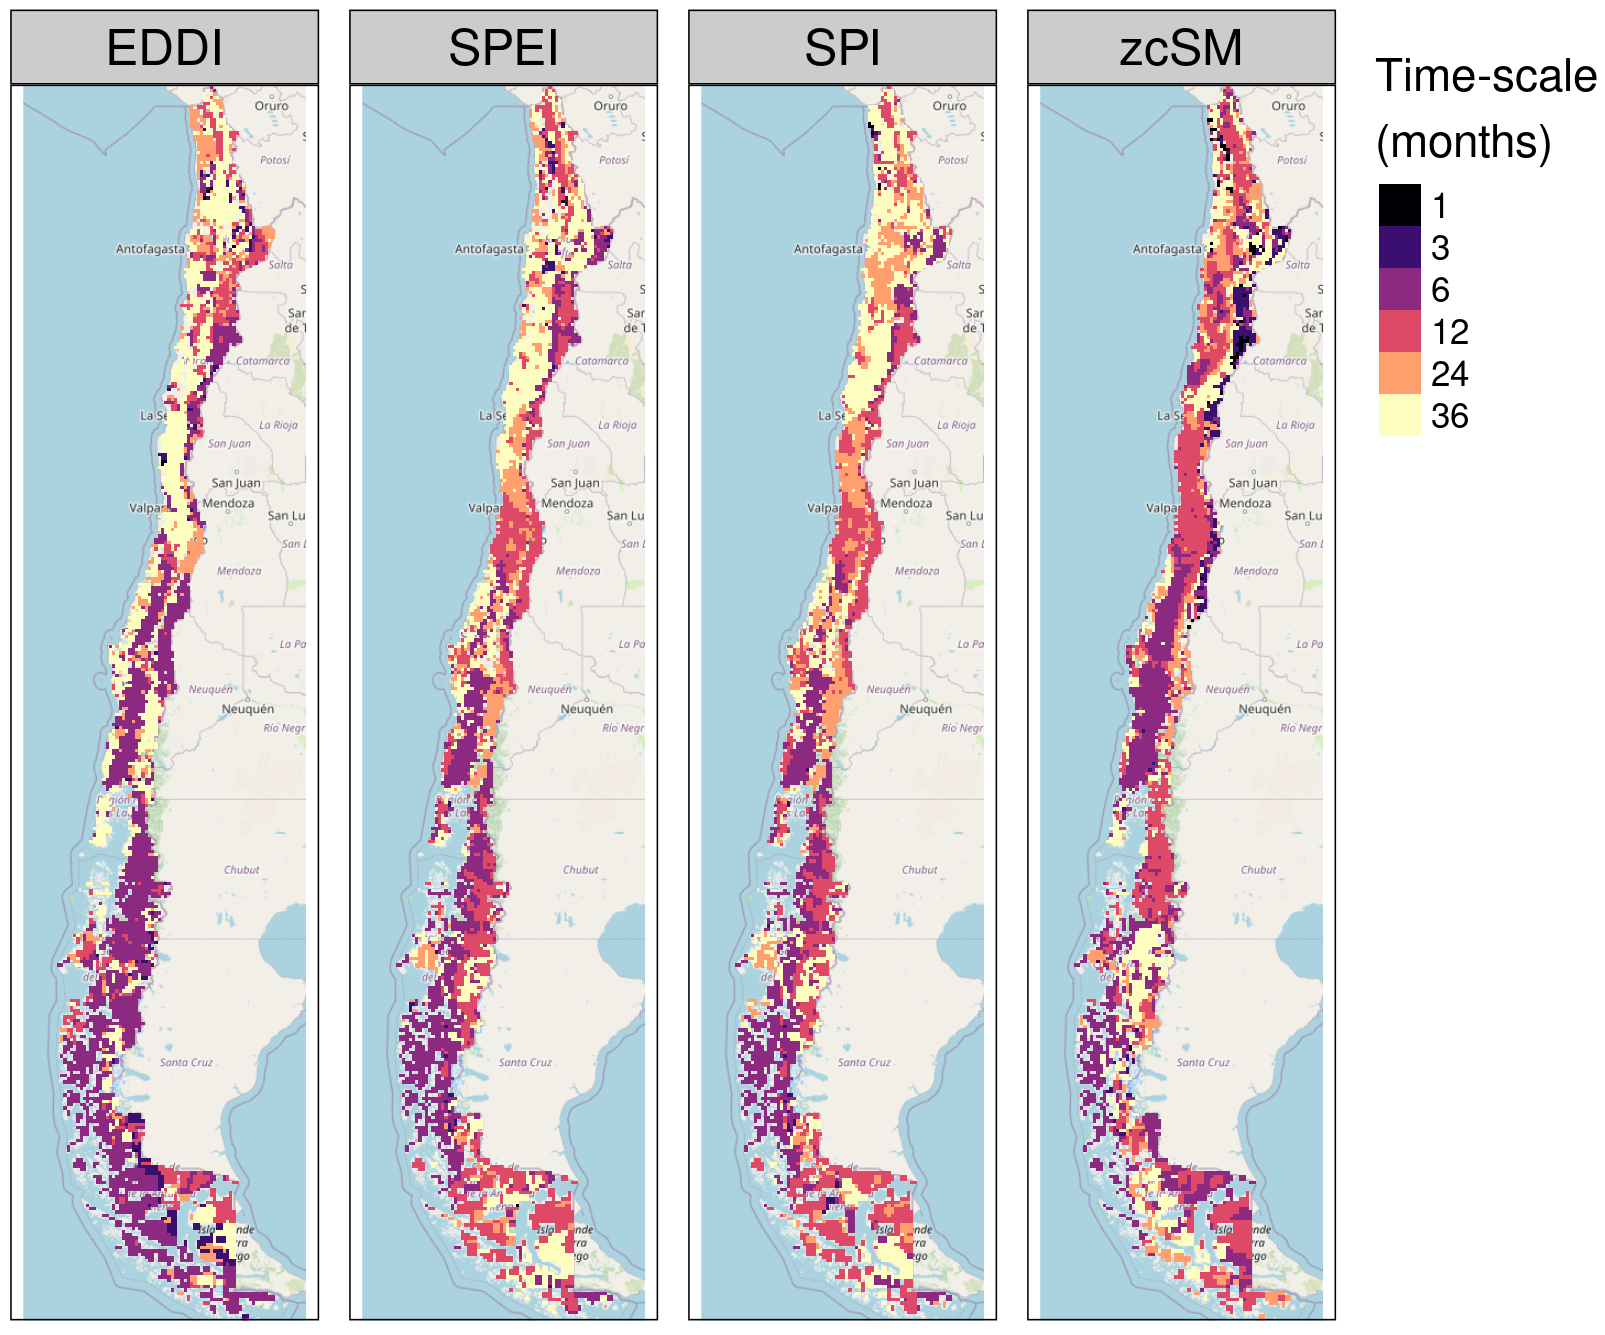
\includegraphics{../output/figs/mapa_cor_selec_indices_zcNDVI6.png}

}

\caption{\label{fig-corTimeScale}Time scales per drought index that
reach the maximum coefficient of determination}

\end{figure}

\begin{figure}[!ht]

{\centering 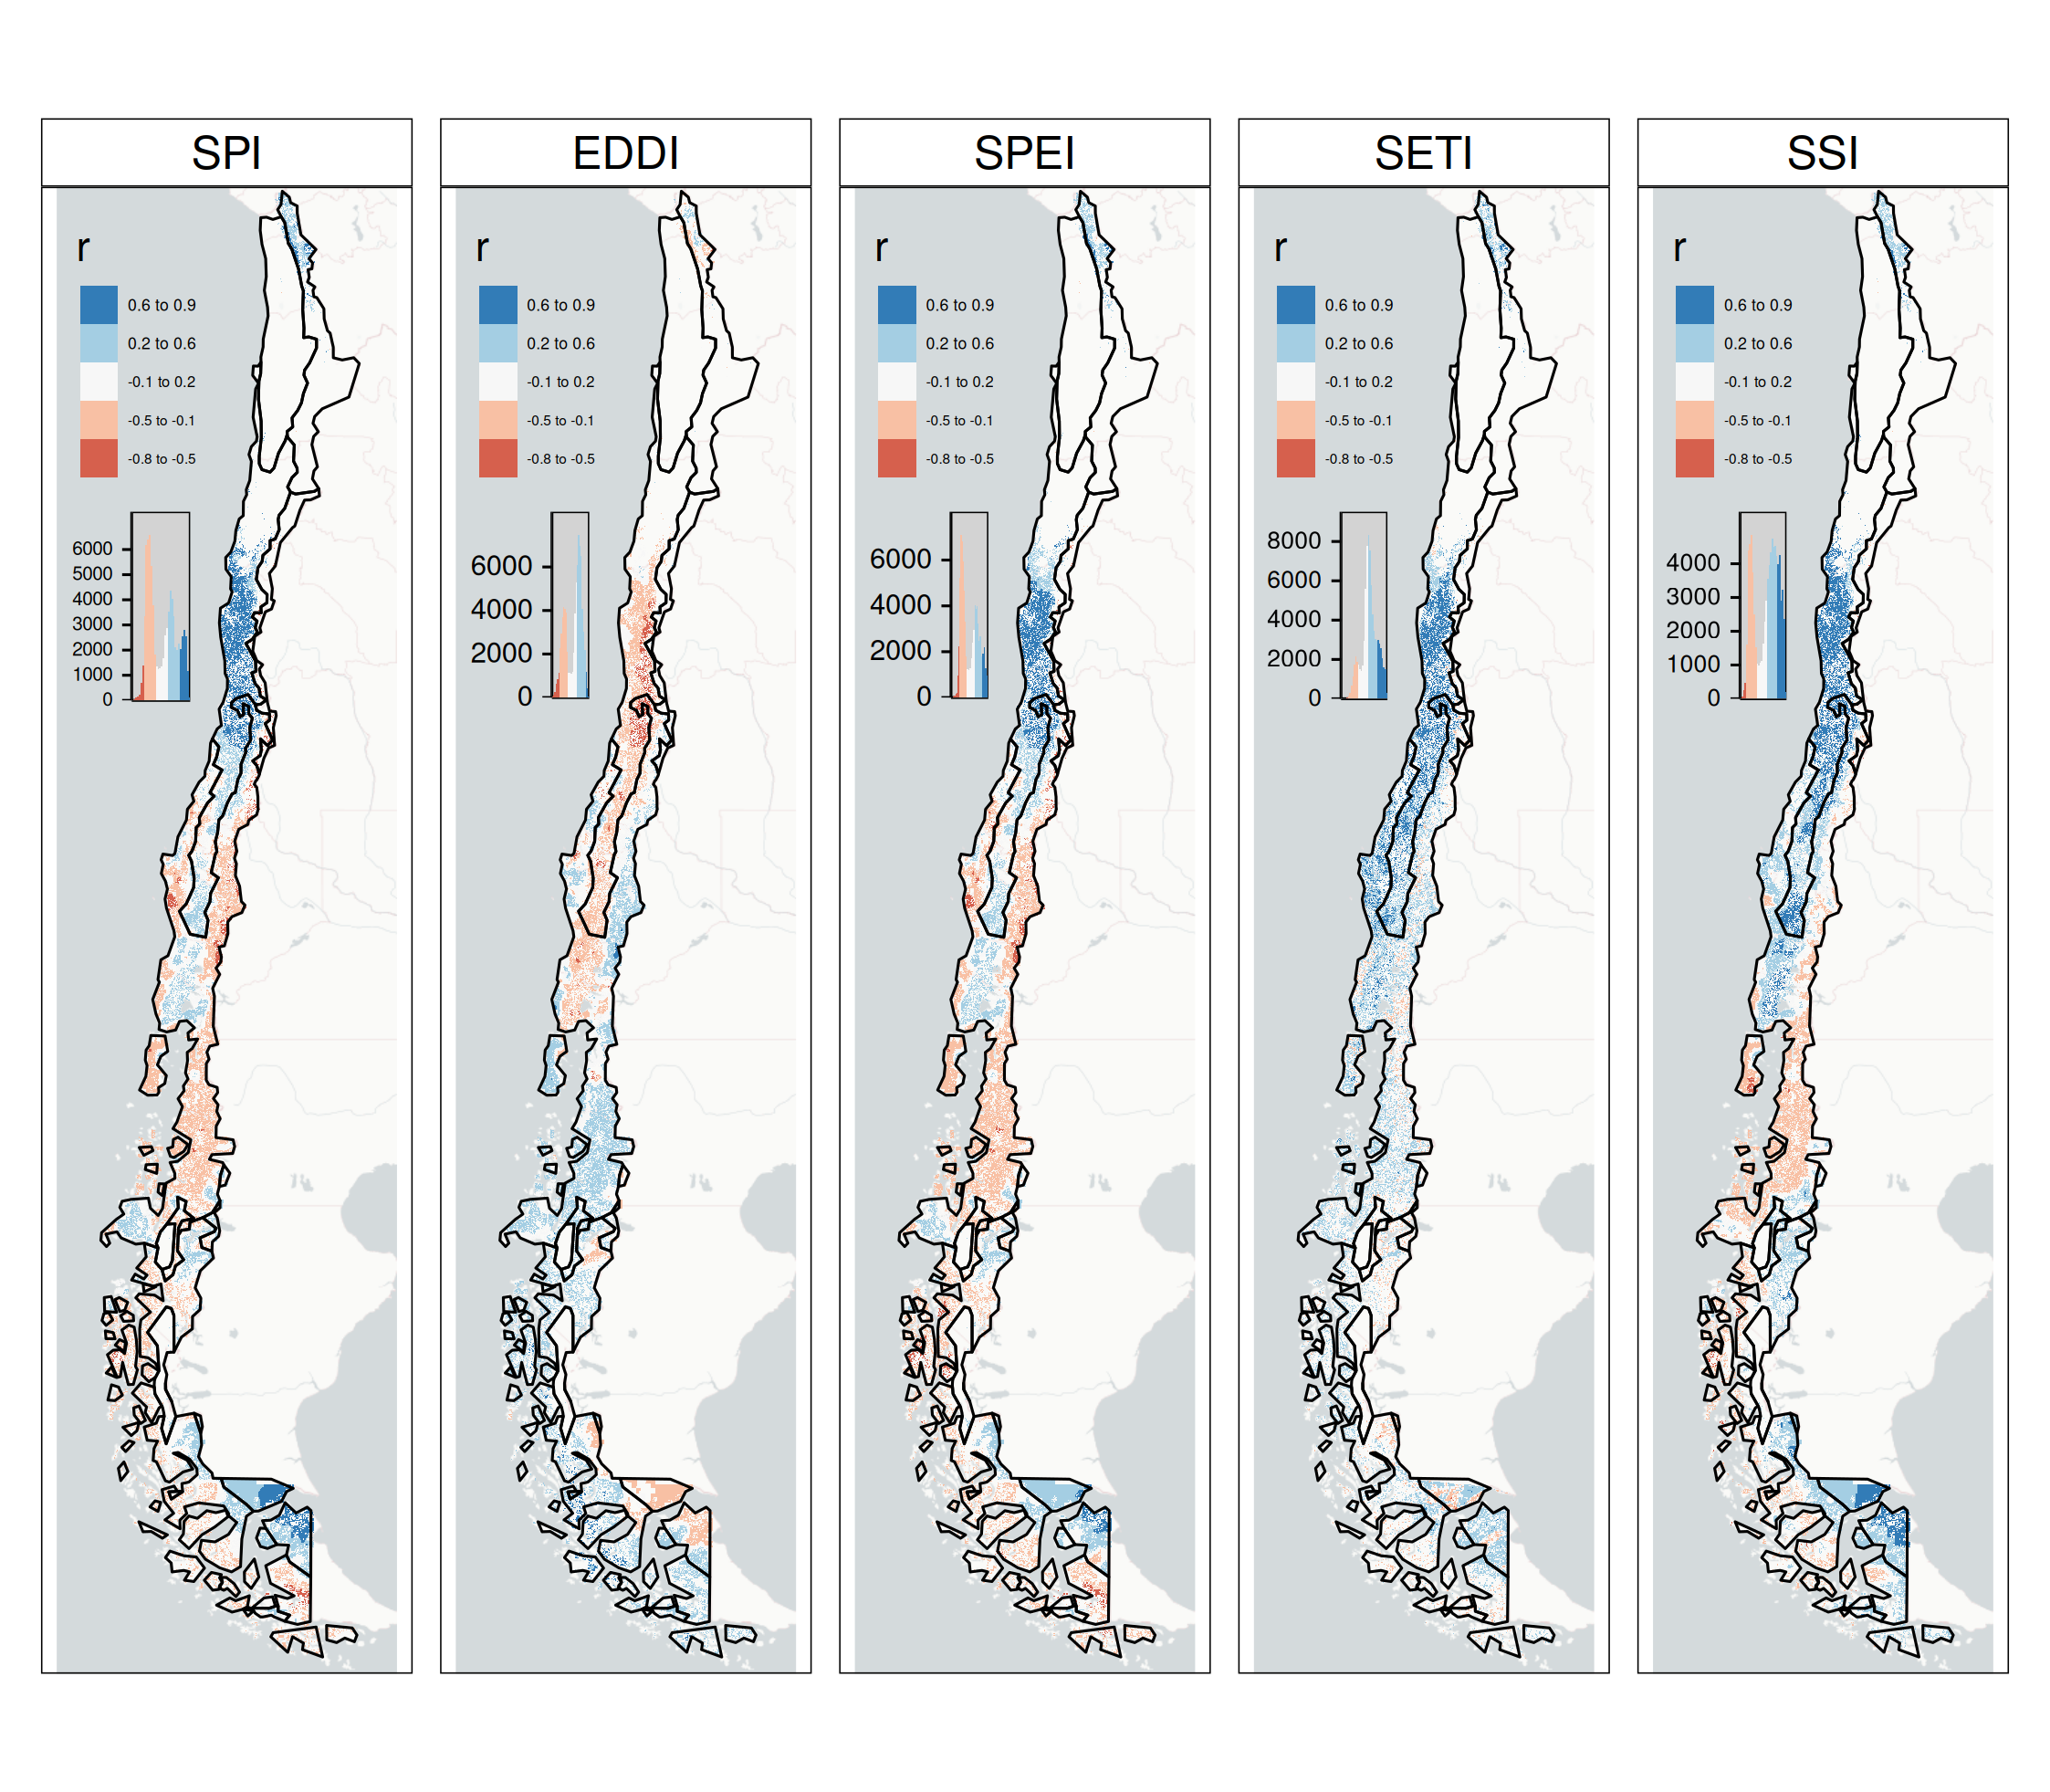
\includegraphics{../output/figs/mapa_cor_r_indices_zcNDVI6.png}

}

\caption{\label{fig-corPerson}Pearson correlation value for the time
scales and drought index that reach the maximum coefficient of
determination}

\end{figure}

\hypertarget{lulc-change-for-2001-2022-and-its-relation-with-water-supply-and-demand-and-soil-moisture}{%
\subsection{LULC change for 2001-2022 and its relation with water supply
and demand, and soil
moisture}\label{lulc-change-for-2001-2022-and-its-relation-with-water-supply-and-demand-and-soil-moisture}}

\begin{table}[!ht]
\label{tab-landcoverTrend}
\caption{Value of linear change trend next to time-series plot of surface, per landcover class (IGBP MCD12Q1.006) for 2001-2019 through Central Chile. Red dots on the plots indicate the maximum and minimum surface}
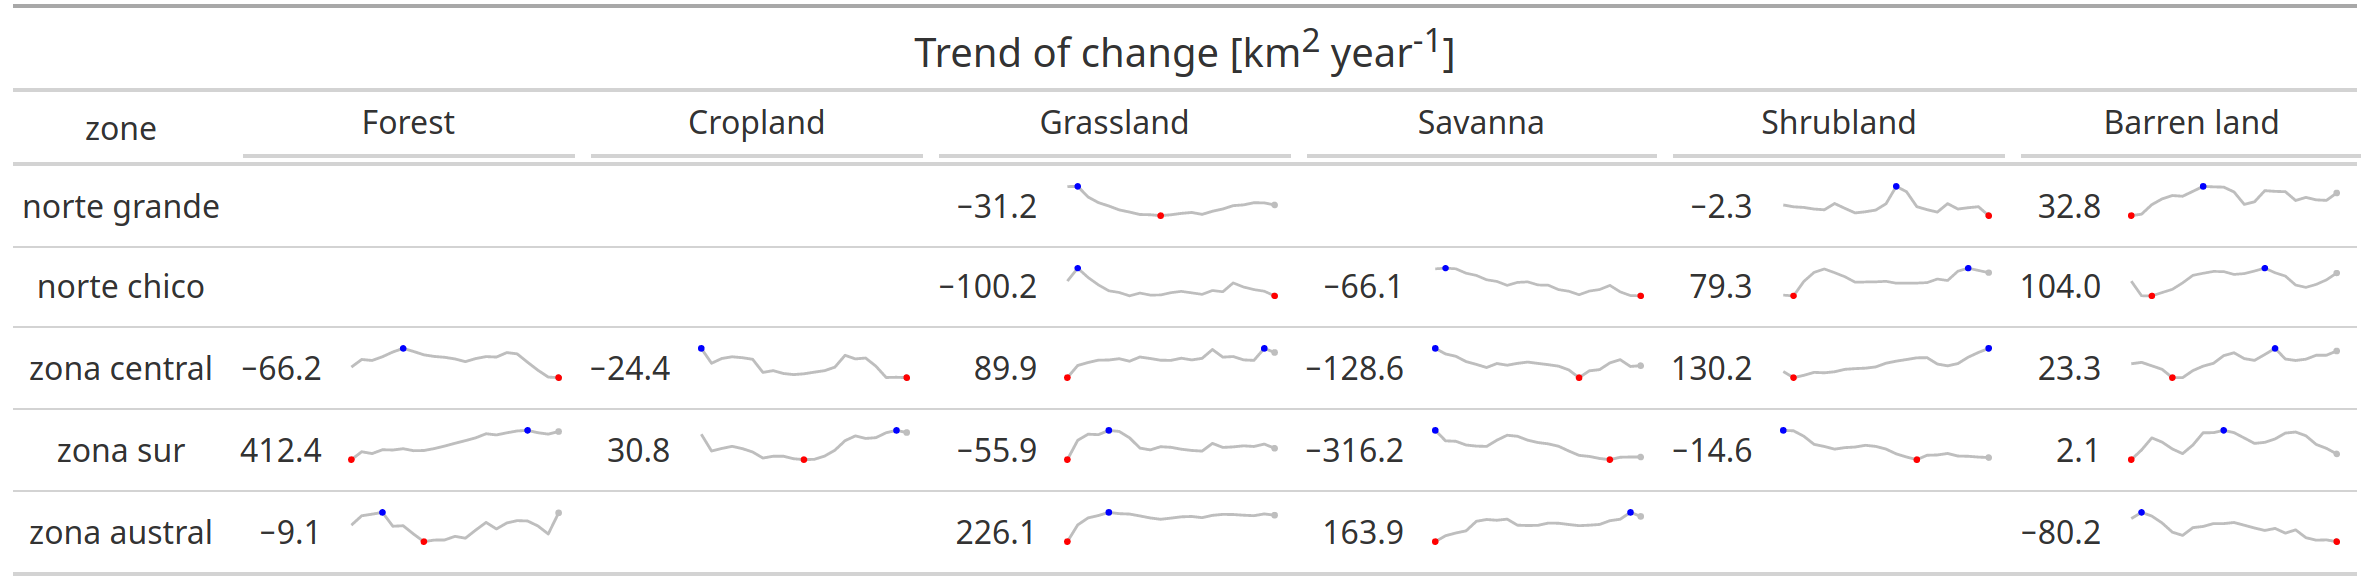
\includegraphics[]{../output/figs/table_var_landcover_macro.png}
\end{table}

\begin{table}[!ht]
\label{tab-corLandcover}
\caption{}
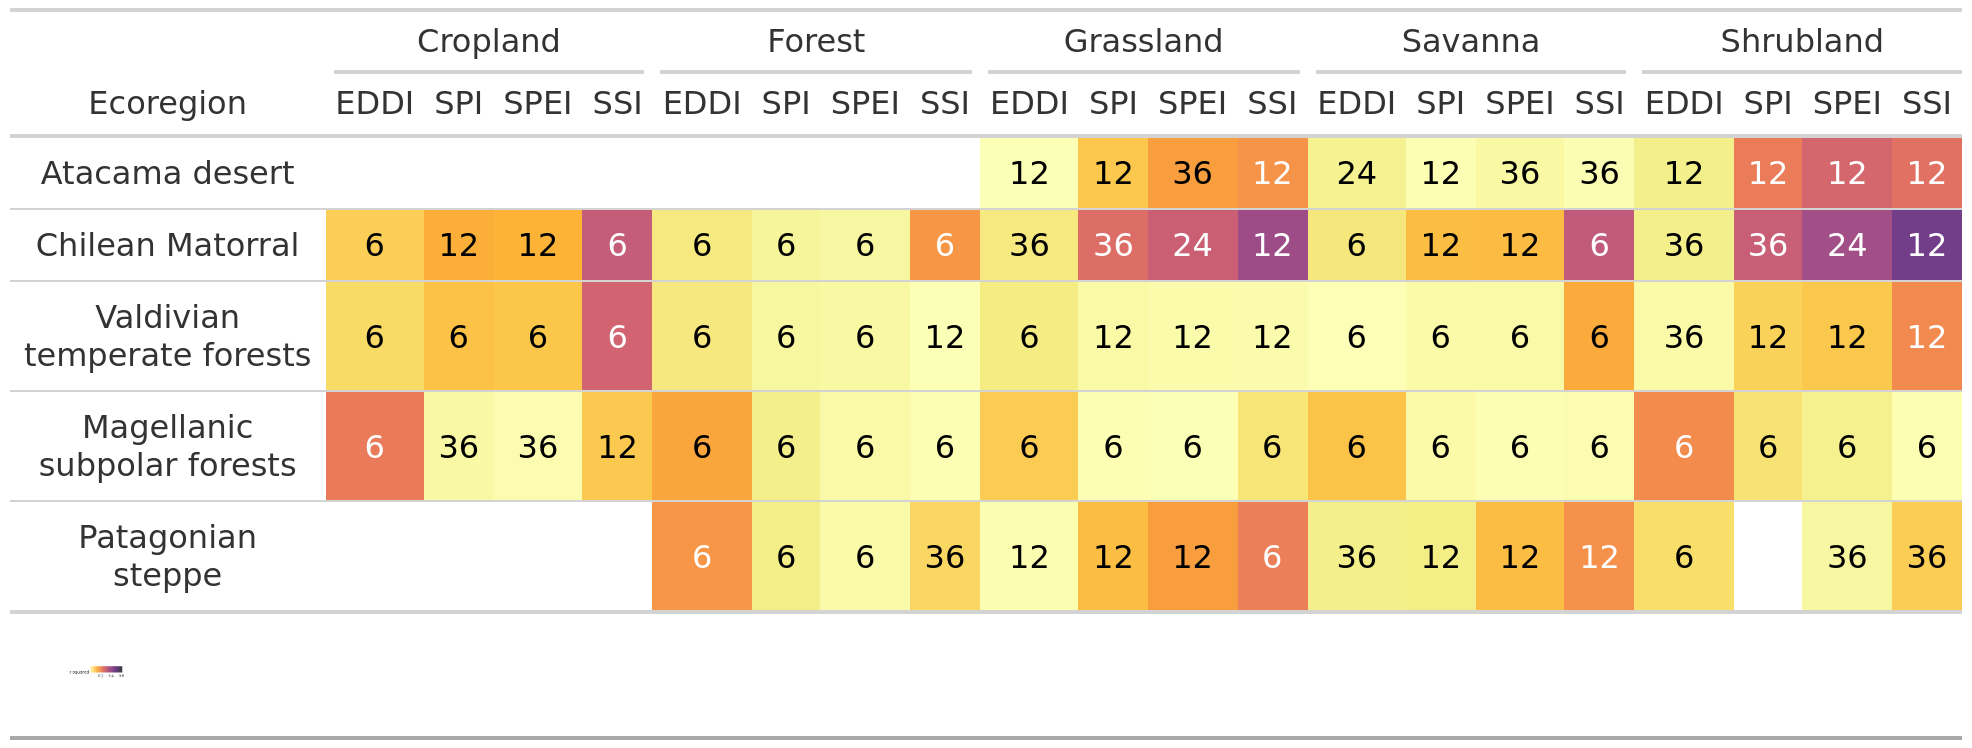
\includegraphics[]{../output/figs/tabla_r_cor_macro_indice.png}
\end{table}

\hypertarget{total-water-storage-tws-and-drought-indices}{%
\subsection{Total water storage (TWS) and drought
indices}\label{total-water-storage-tws-and-drought-indices}}

\hypertarget{validation-of-era5-land-variables-1}{%
\subsection{Validation of ERA5-Land
variables}\label{validation-of-era5-land-variables-1}}

\hypertarget{discussion}{%
\section{Discussion}\label{discussion}}

\hypertarget{conclusion}{%
\section{Conclusion}\label{conclusion}}


\renewcommand\refname{References}
  \bibliography{references.bib}


\end{document}
